\section{实验步骤}
本实验按照实验手册中的指导进行。主要分为以下步骤:
\begin{enumerate}
    \item 编译构建智慧路灯应用
    \item 创建主题并订阅 SMN
    \item 创建弹性云服务器 ECS
    \item 部署智慧路灯应用
    \item 导入产品模型
    \item 配置智慧路灯应用(订阅推送方案)
    \item 结果验证(设备属性上报/订阅/设备命令下发)
\end{enumerate}

下面展示的是实验中的关键步骤的截图。

\begin{figure}[!htbp]
\centering
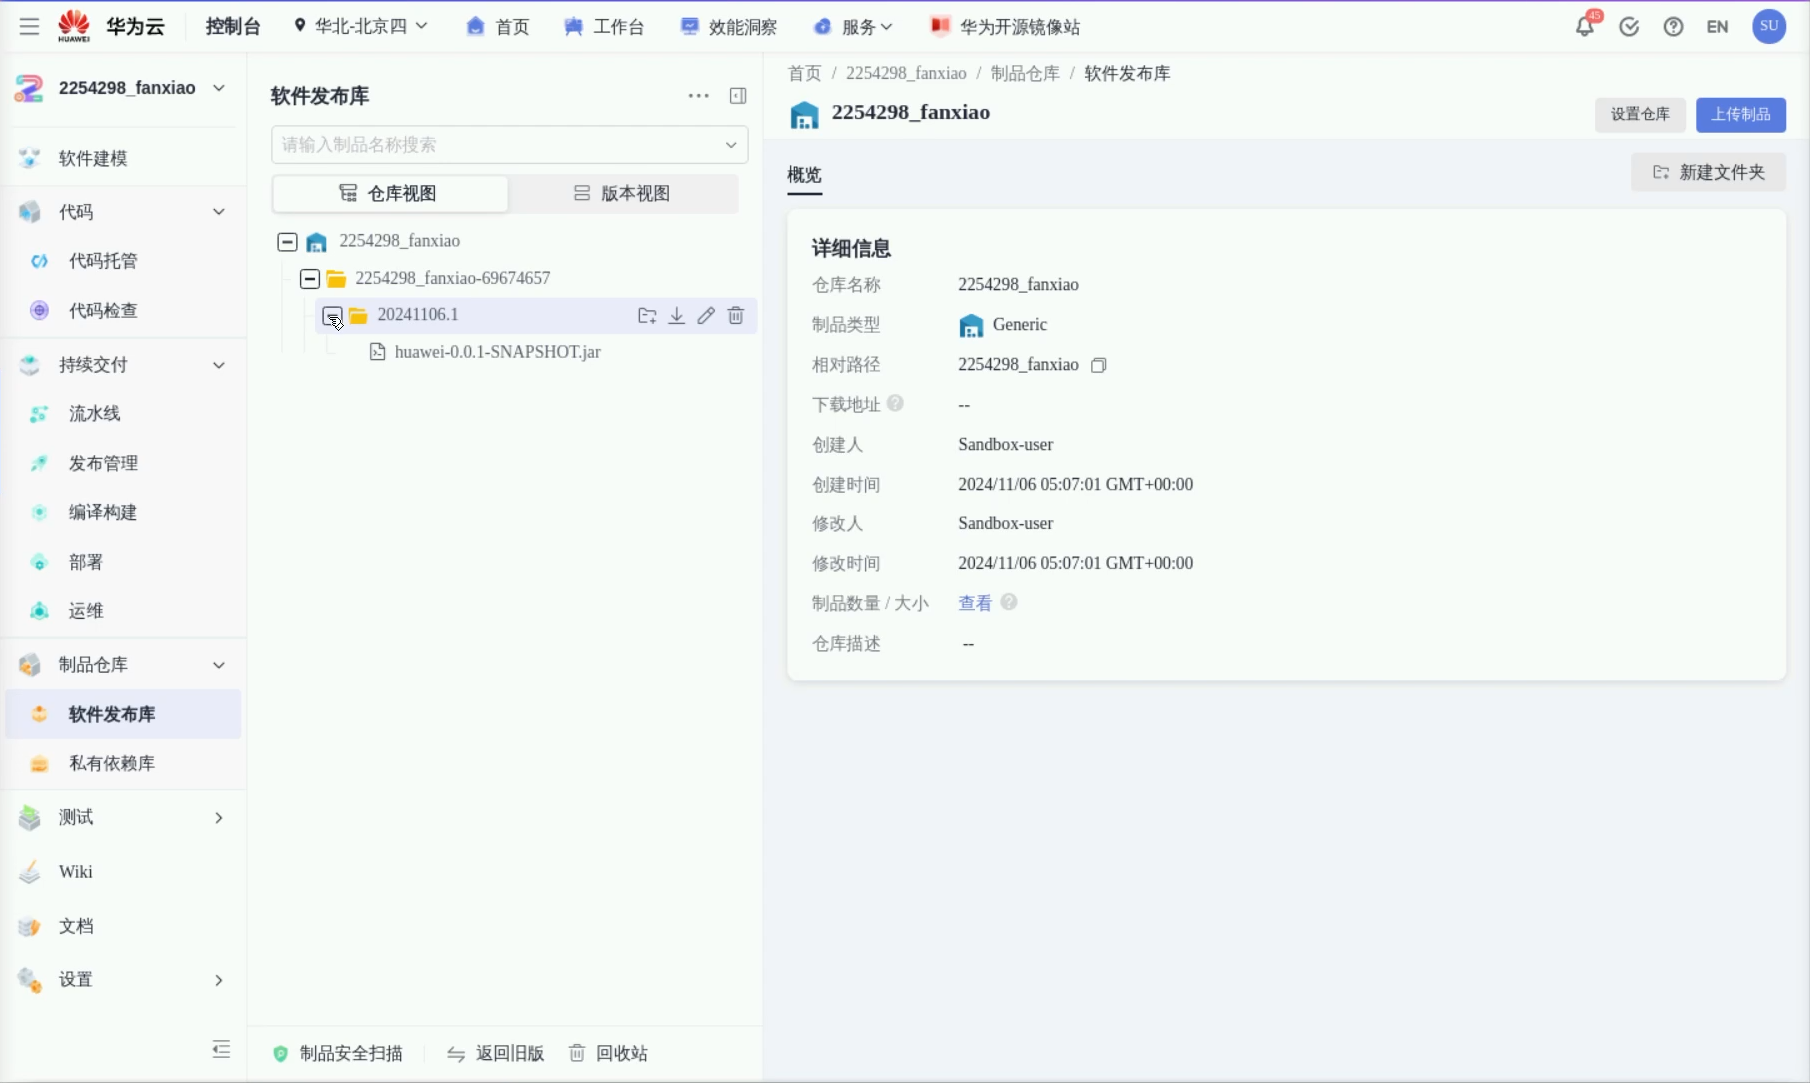
\includegraphics[width=\textwidth]{figures/序列 01.00_00_12_39.Still003.png}
\caption{成功构建智慧路灯应用}\label{成功构建智慧路灯应用}
\end{figure}

\begin{figure}[!htbp]
\centering
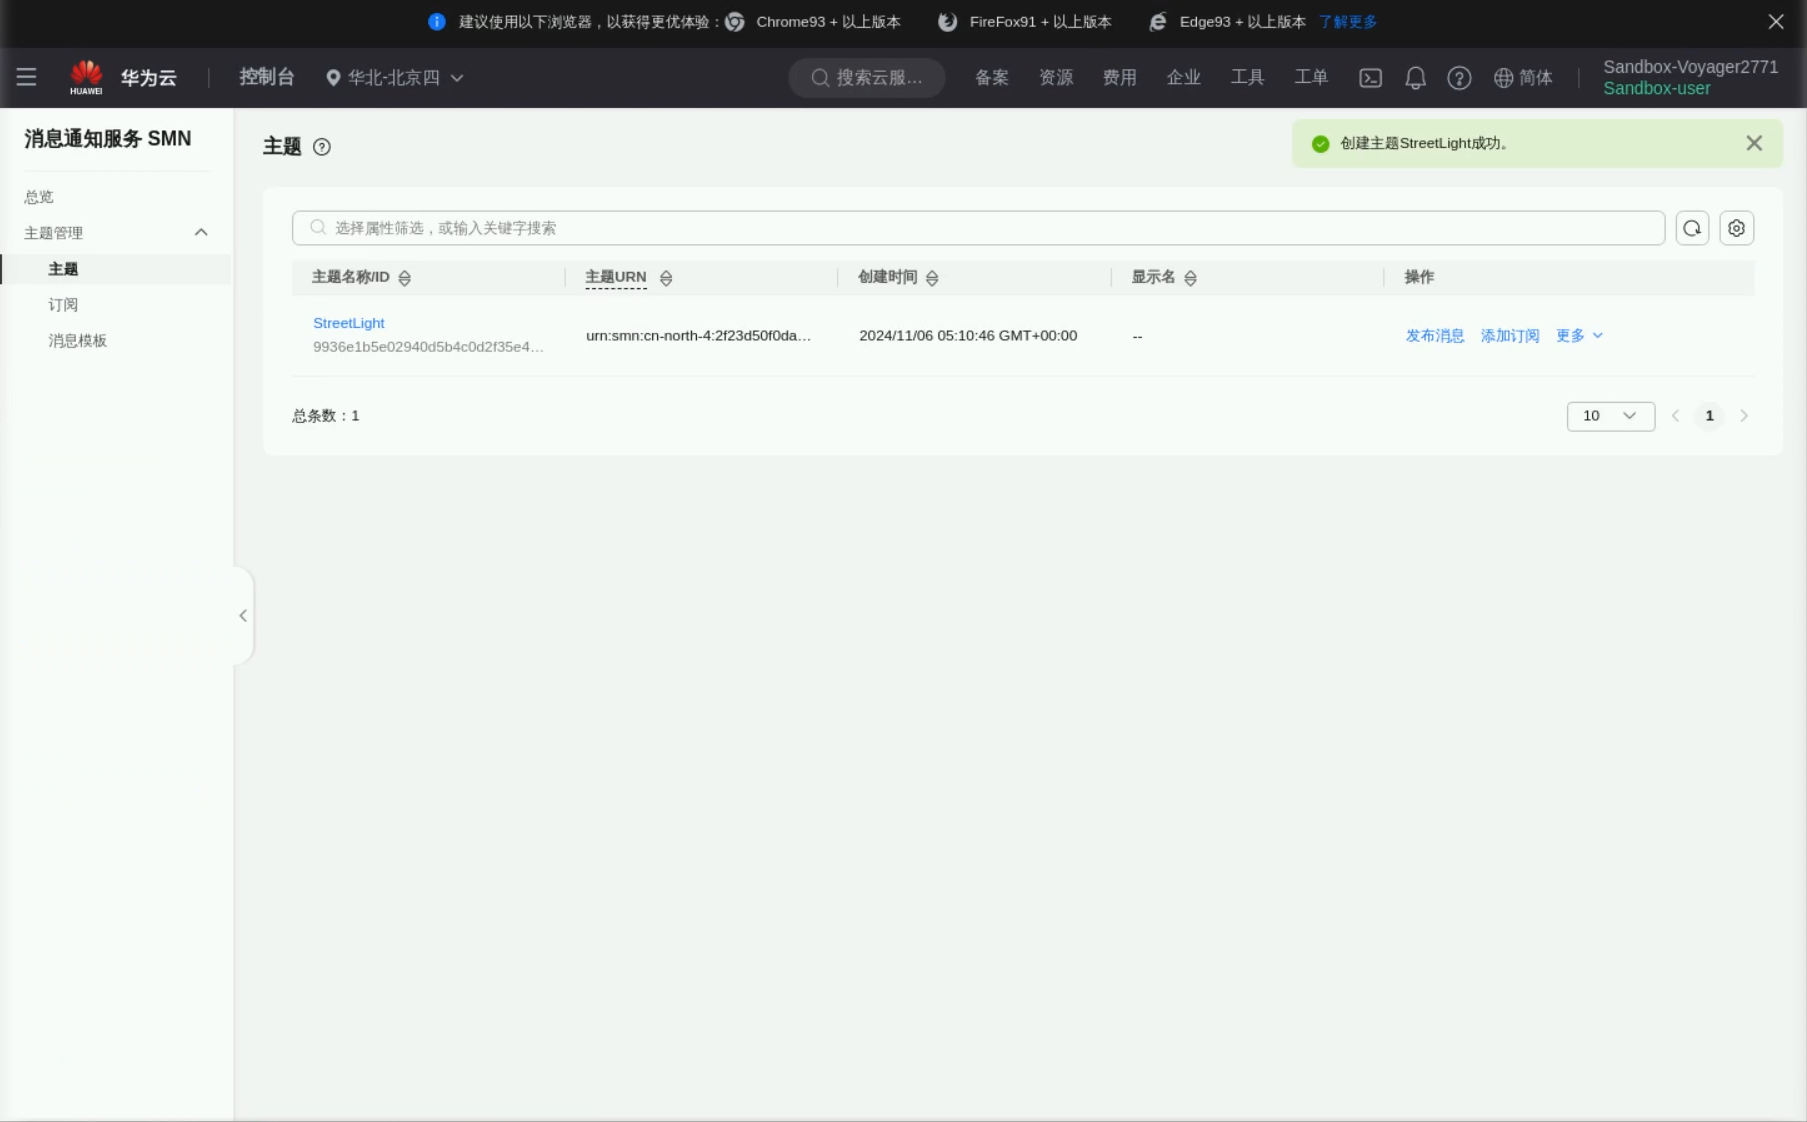
\includegraphics[width=\textwidth]{figures/序列 01.00_01_23_17.Still004.png}
\caption{成功创建SMN主题}\label{成功创建SMN主题}
\end{figure}

\begin{figure}[!htbp]
\centering
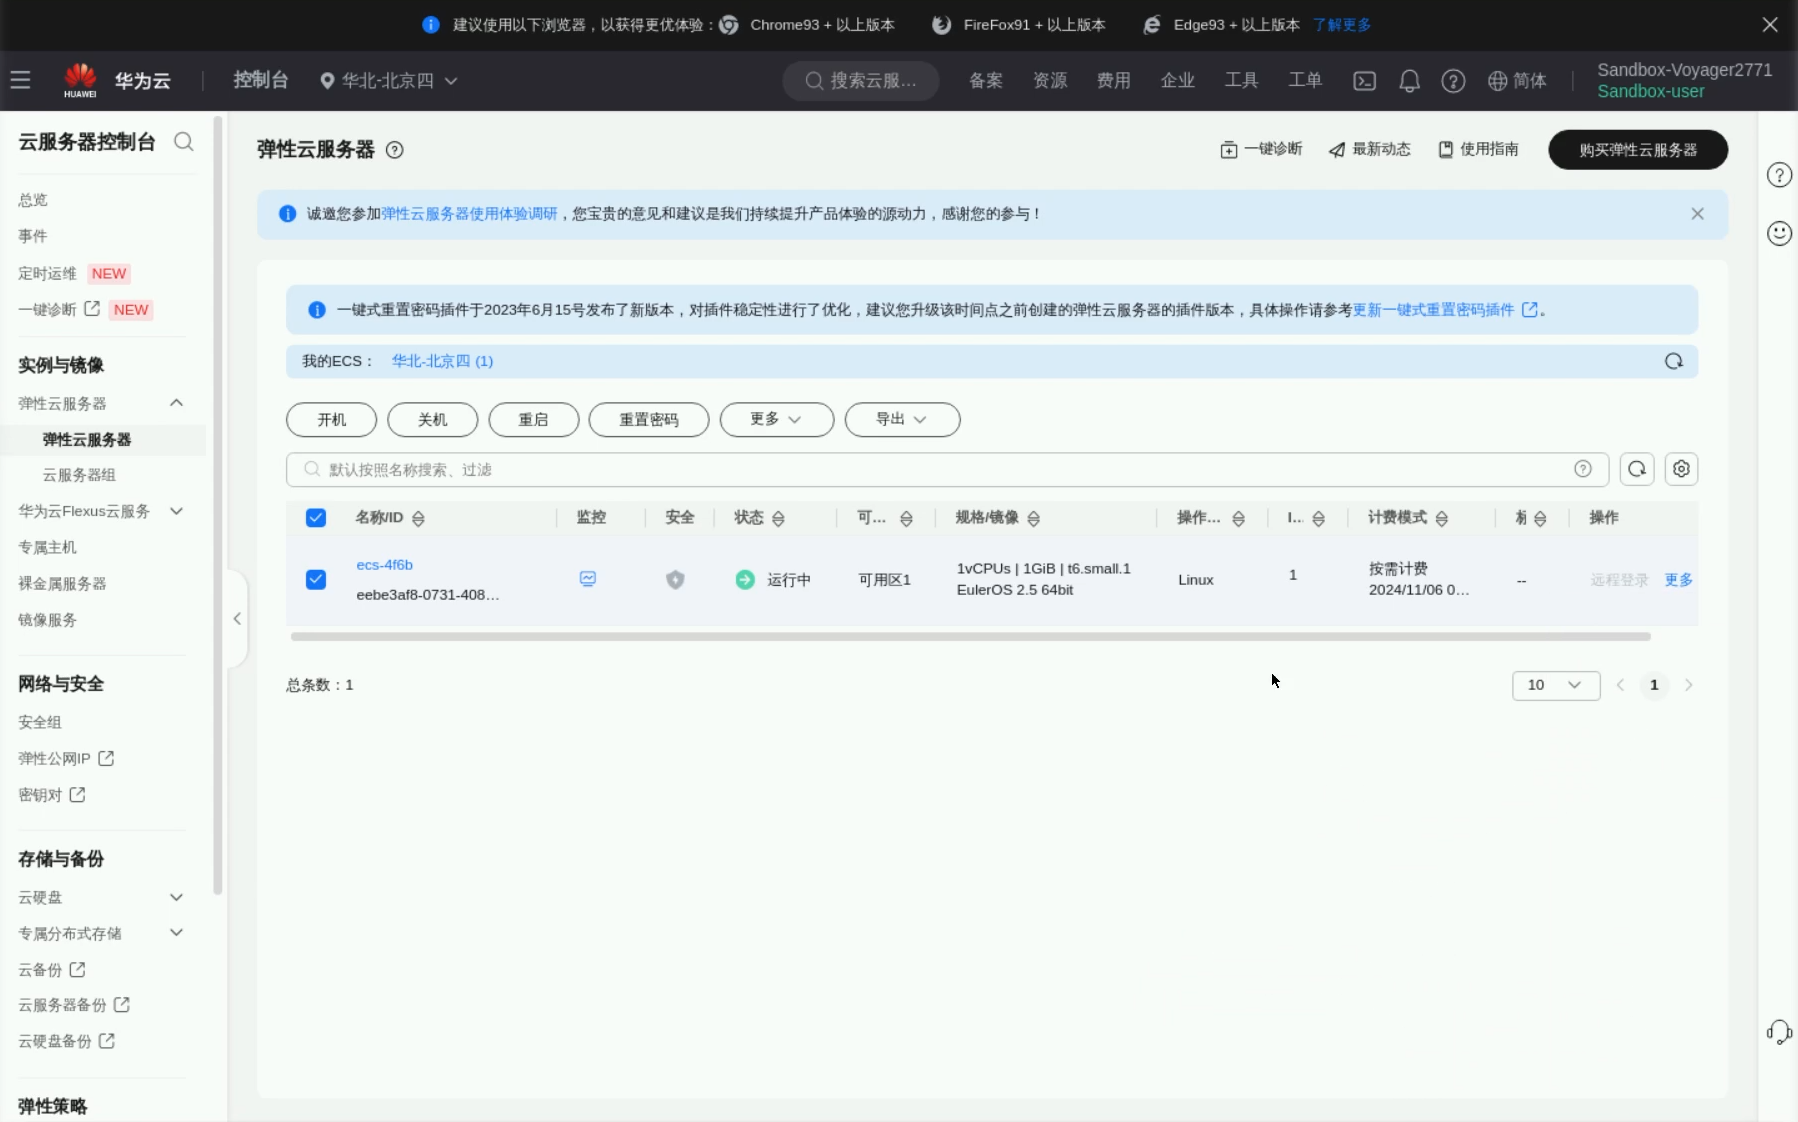
\includegraphics[width=\textwidth]{figures/序列 01.00_05_06_39.Still005.png}
\caption{成功创建弹性云服务器ECS}\label{成功创建弹性云服务器ECS}
\end{figure}

\begin{figure}[!htbp]
\centering
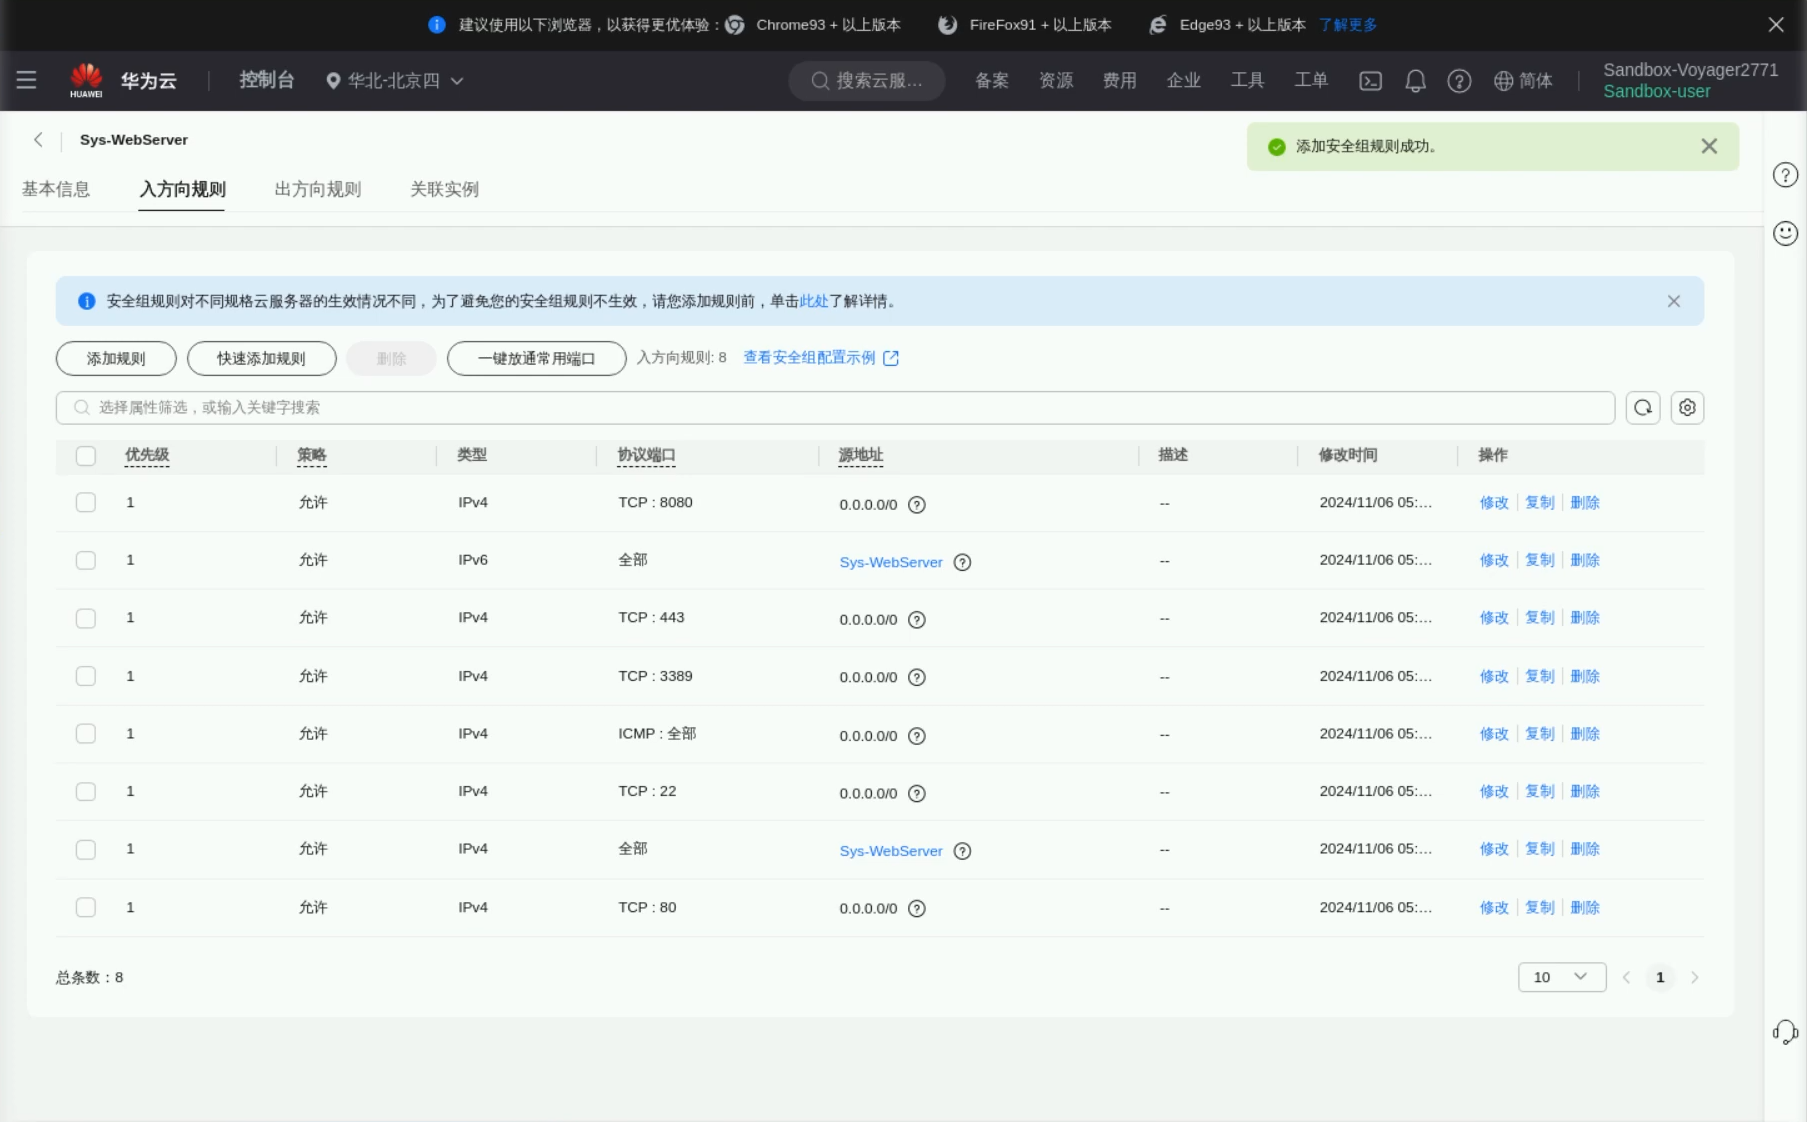
\includegraphics[width=\textwidth]{figures/序列 01.00_05_44_31.Still006.png}
\caption{配置网络安全组}\label{配置网络安全组}
\end{figure}

\begin{figure}[!htbp]
\centering
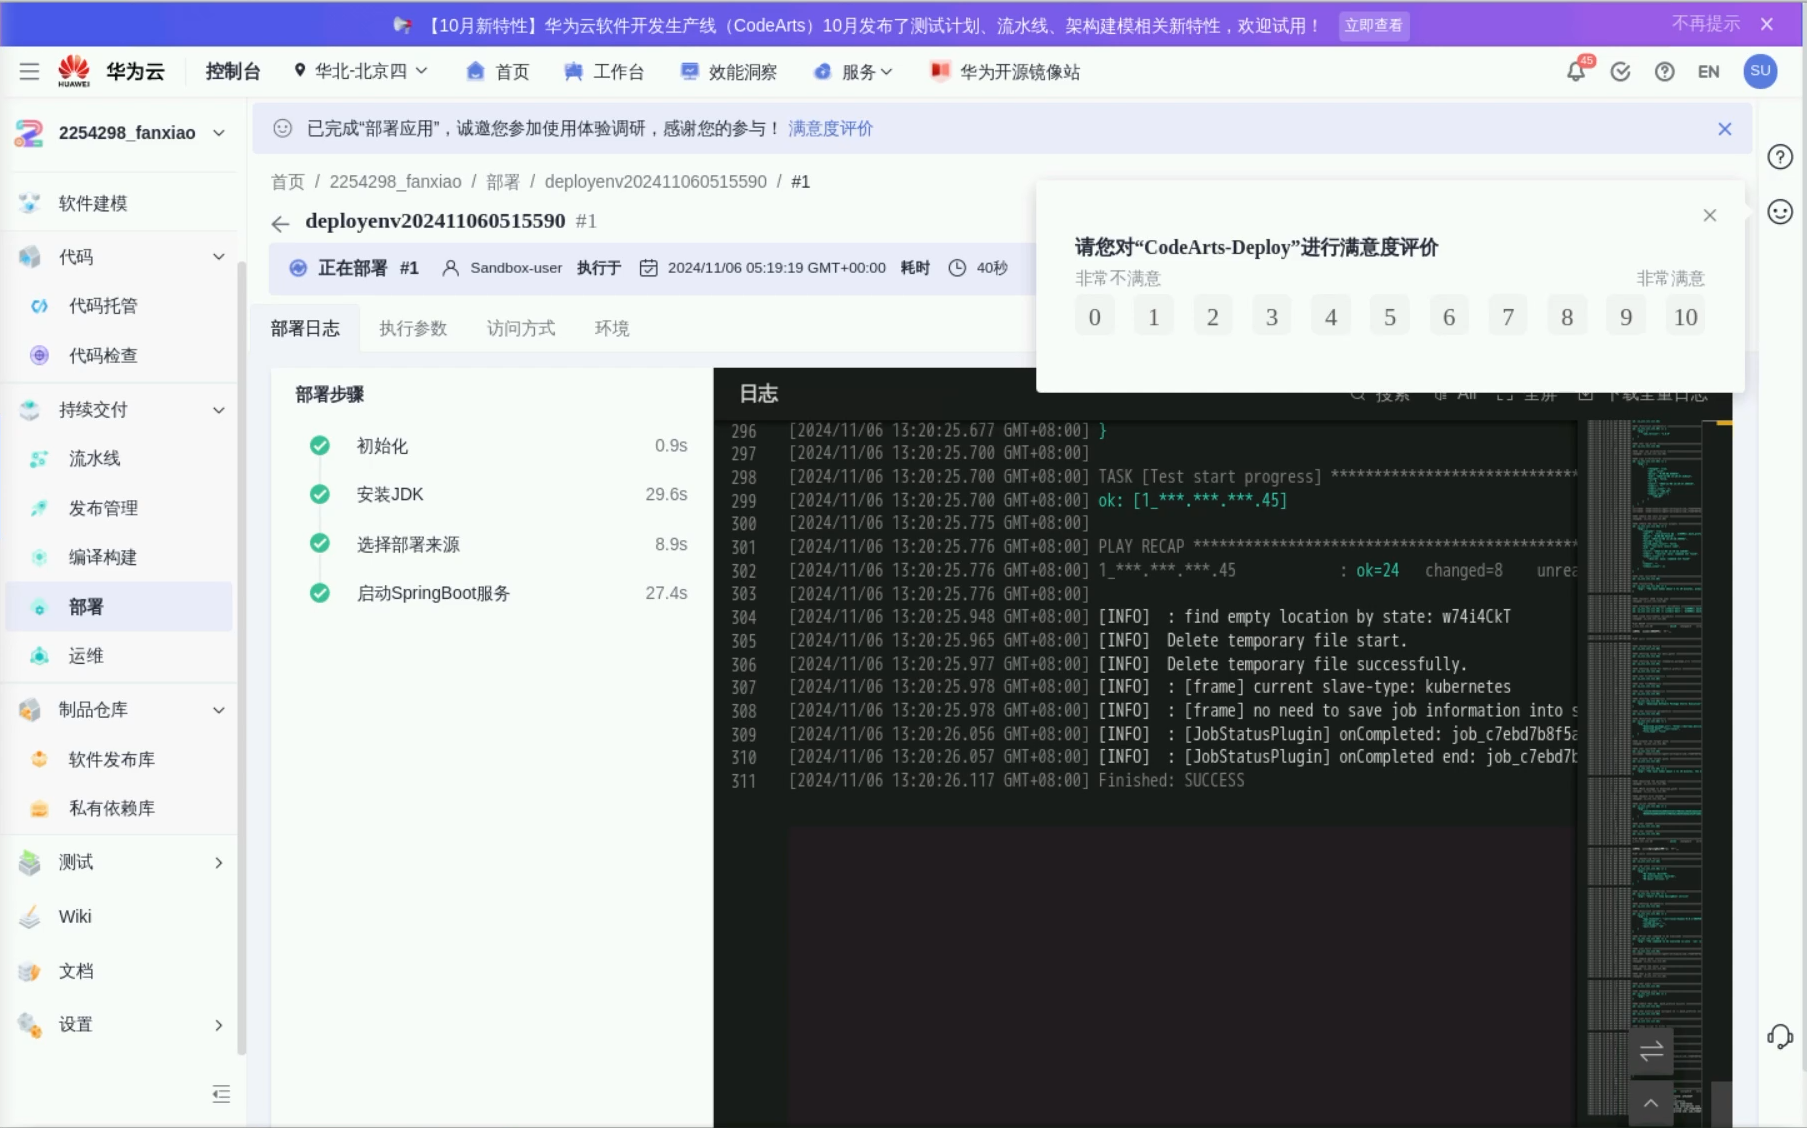
\includegraphics[width=\textwidth]{figures/序列 01.00_11_19_34.Still007.png}
\caption{成功部署智慧路灯应用}\label{成功部署智慧路灯应用}
\end{figure}

\begin{figure}[!htbp]
\centering
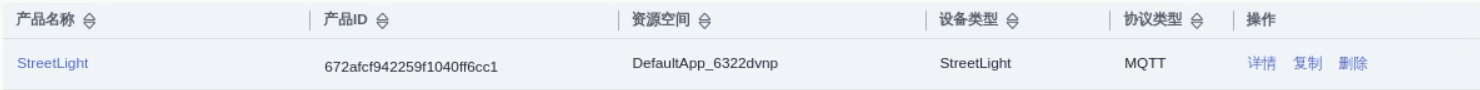
\includegraphics[width=\textwidth]{figures/序列 01.00_12_42_51.Still008.png}
\caption{成功导入产品模型}\label{成功导入产品模型}
\end{figure}

\begin{figure}[!htbp]
\centering
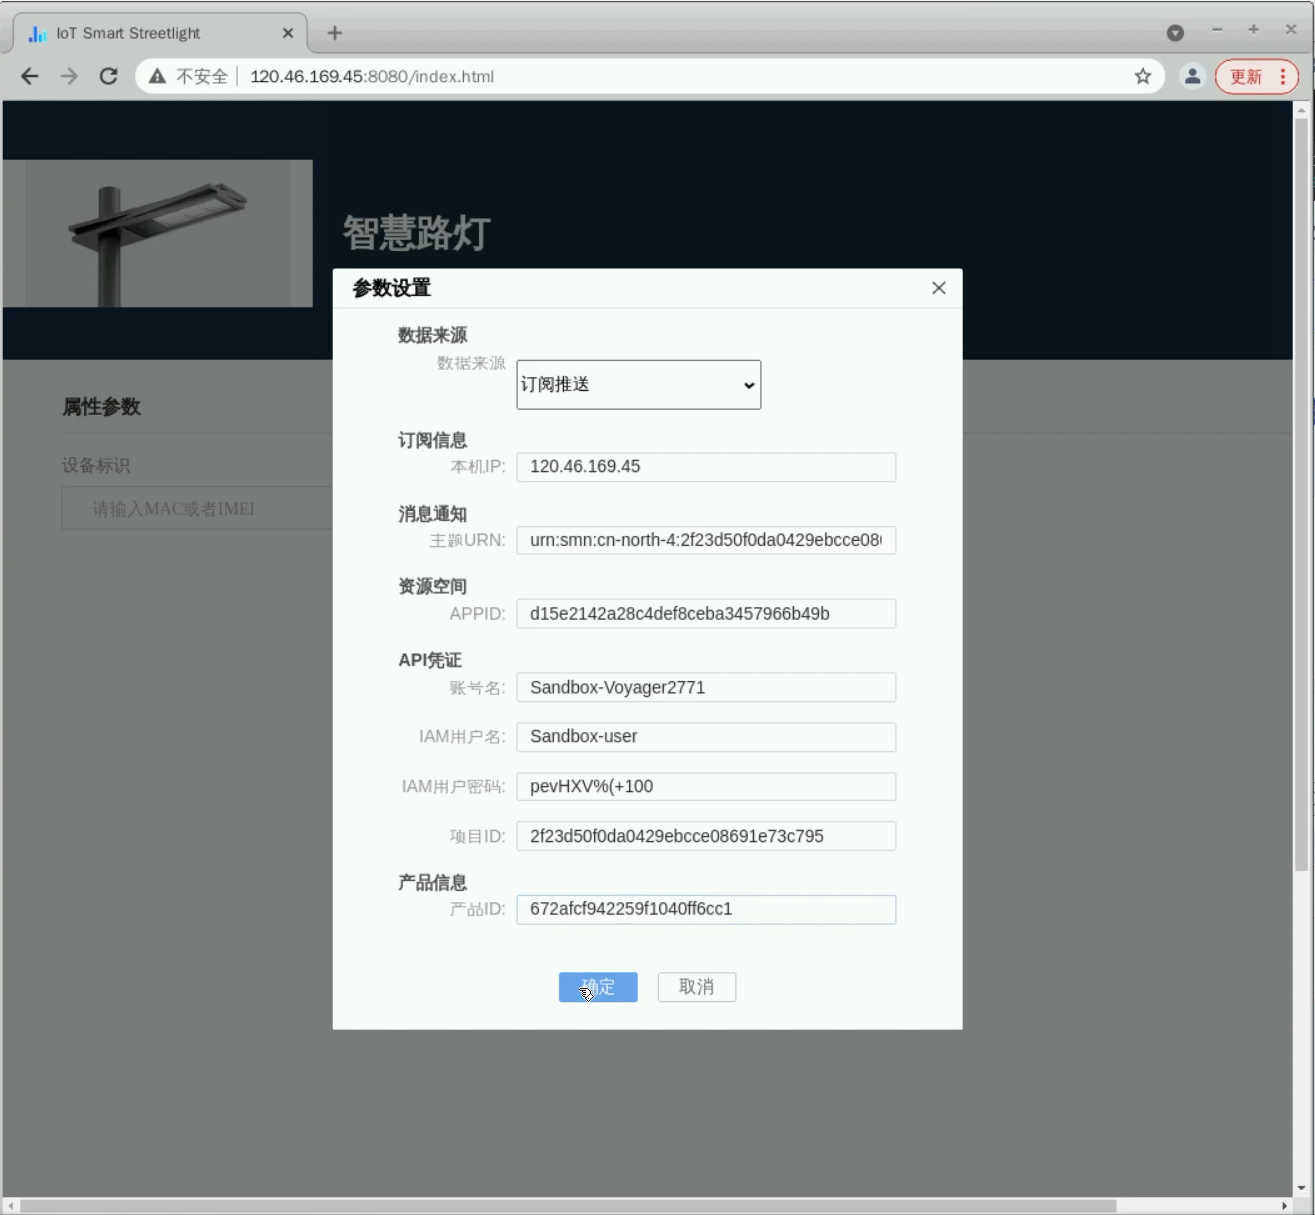
\includegraphics[width=\textwidth]{figures/序列 01.00_15_17_06.Still009.png}
\caption{成功配置智慧路灯应用}\label{成功配置智慧路灯应用}
\end{figure}

\begin{figure}[!htbp]
\centering
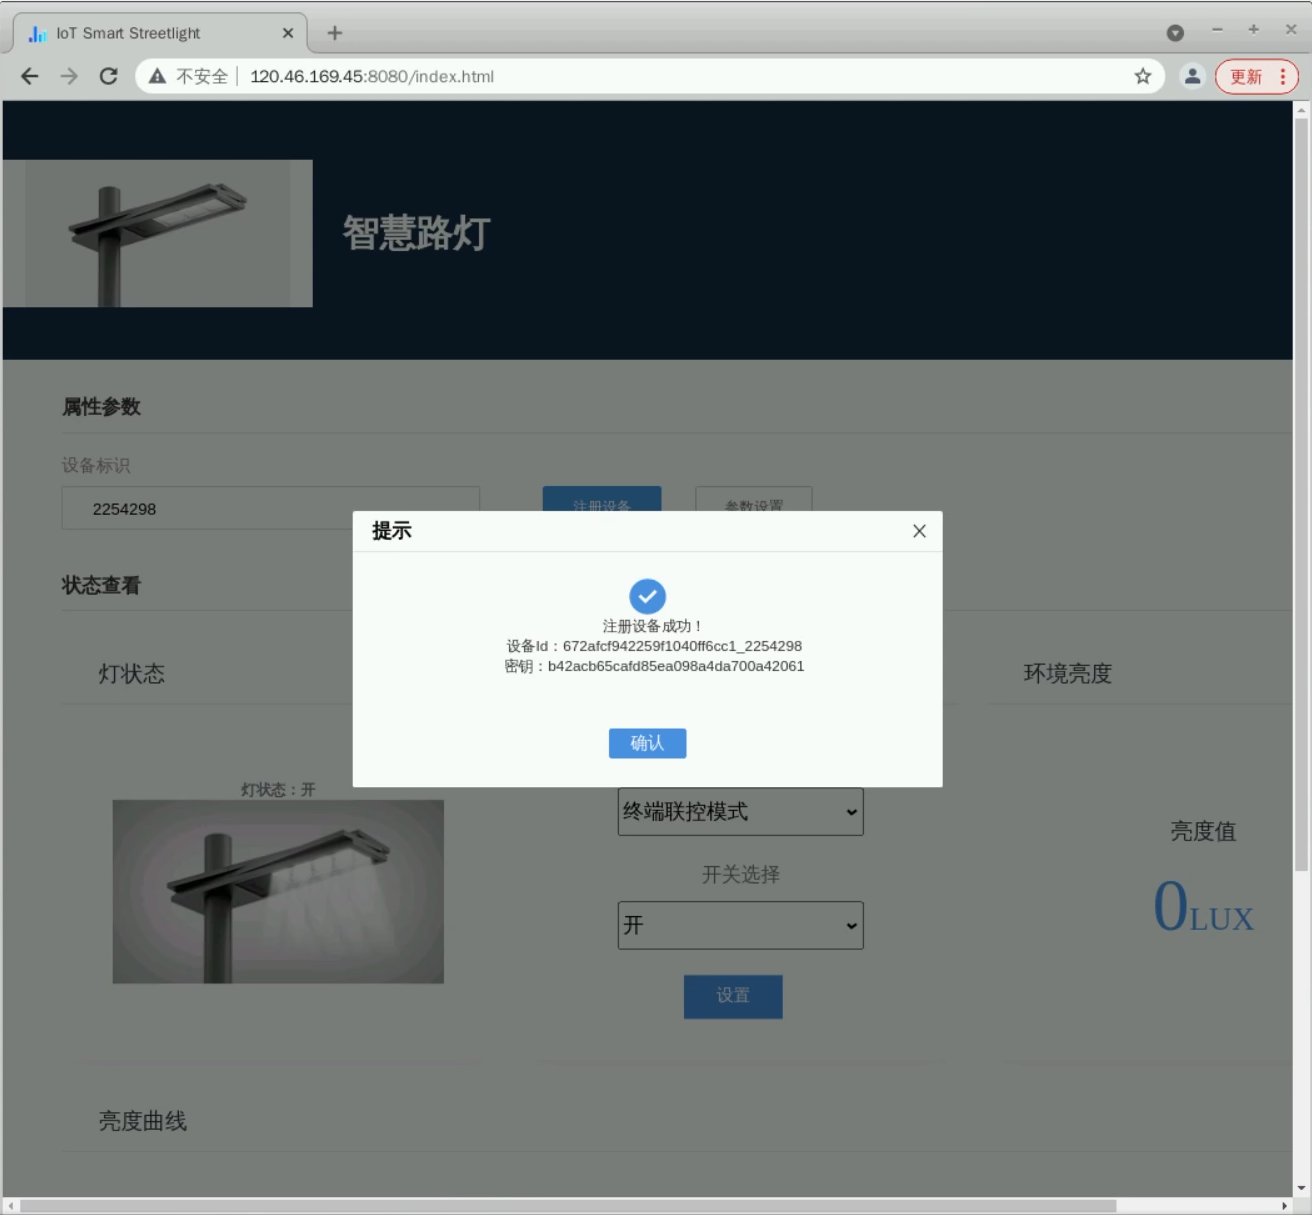
\includegraphics[width=\textwidth]{figures/序列 01.00_15_33_13.Still010.png}
\caption{注册设备成功}\label{注册设备成功}
\end{figure}

\begin{figure}[!htbp]
\centering
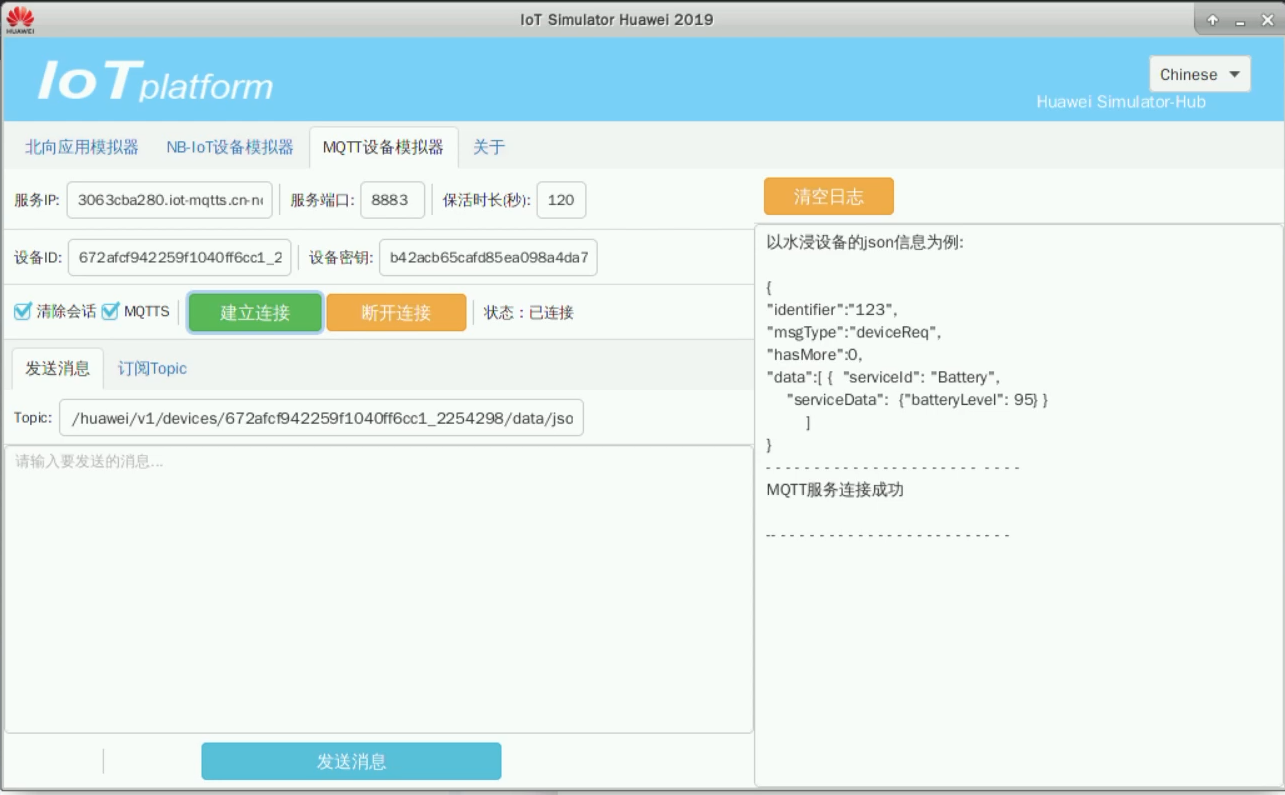
\includegraphics[width=\textwidth]{figures/序列 01.00_18_16_00.Still011.png}
\caption{模拟器页面}\label{模拟器页面}
\end{figure}

\begin{figure}[!htbp]
\centering
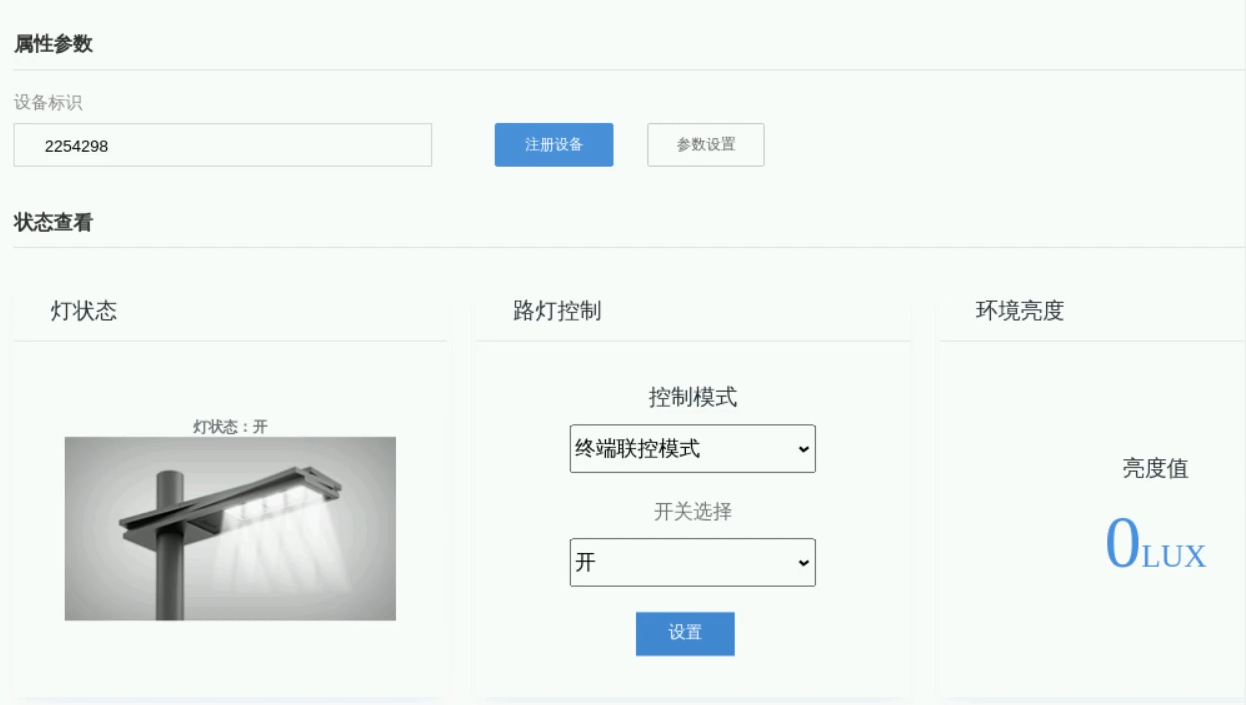
\includegraphics[width=\textwidth]{figures/序列 01.00_19_20_22.Still012.png}
\caption{智慧路灯应用初始页面}\label{智慧路灯应用初始页面}
\end{figure}

\begin{figure}[!htbp]
\centering
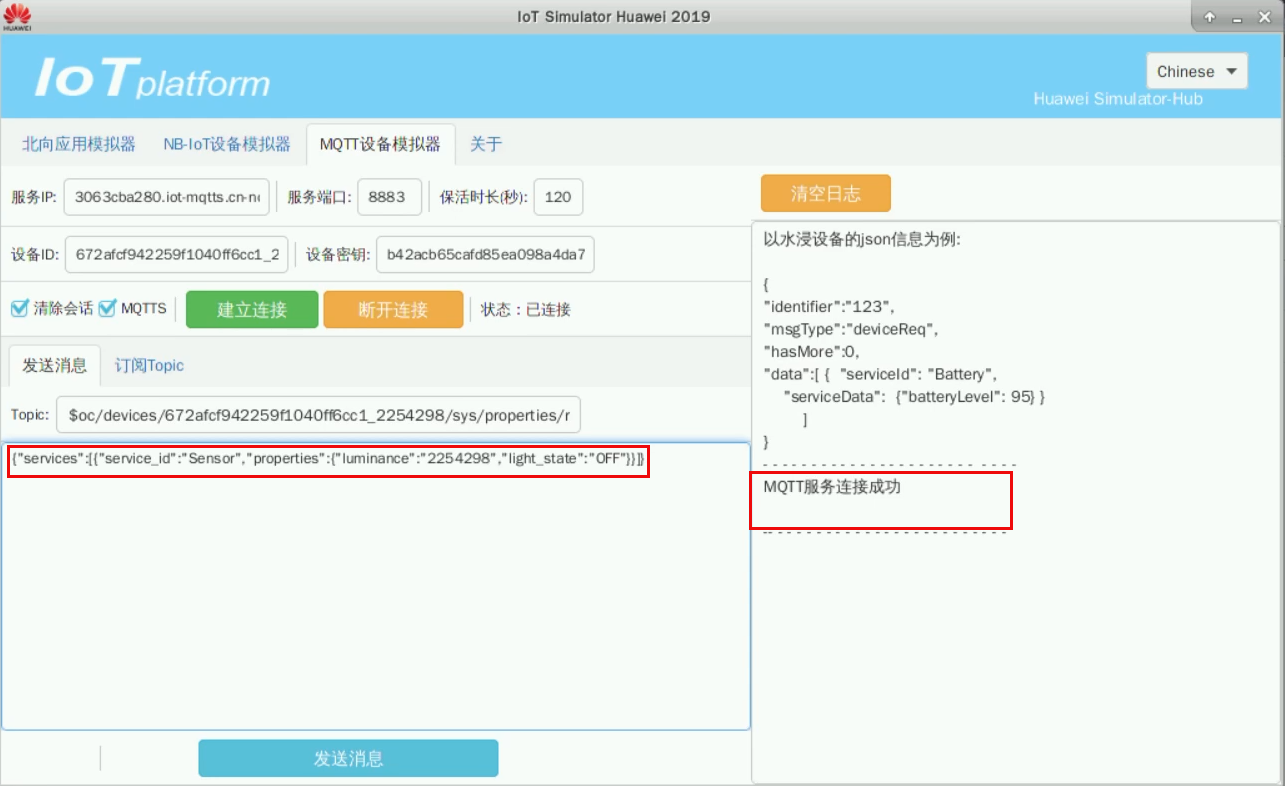
\includegraphics[width=\textwidth]{figures/序列 01.00_19_35_30.Still013.png}
\caption{成功连接MQTT服务}\label{成功连接MQTT服务}
\end{figure}

\begin{figure}[!htbp]
\centering
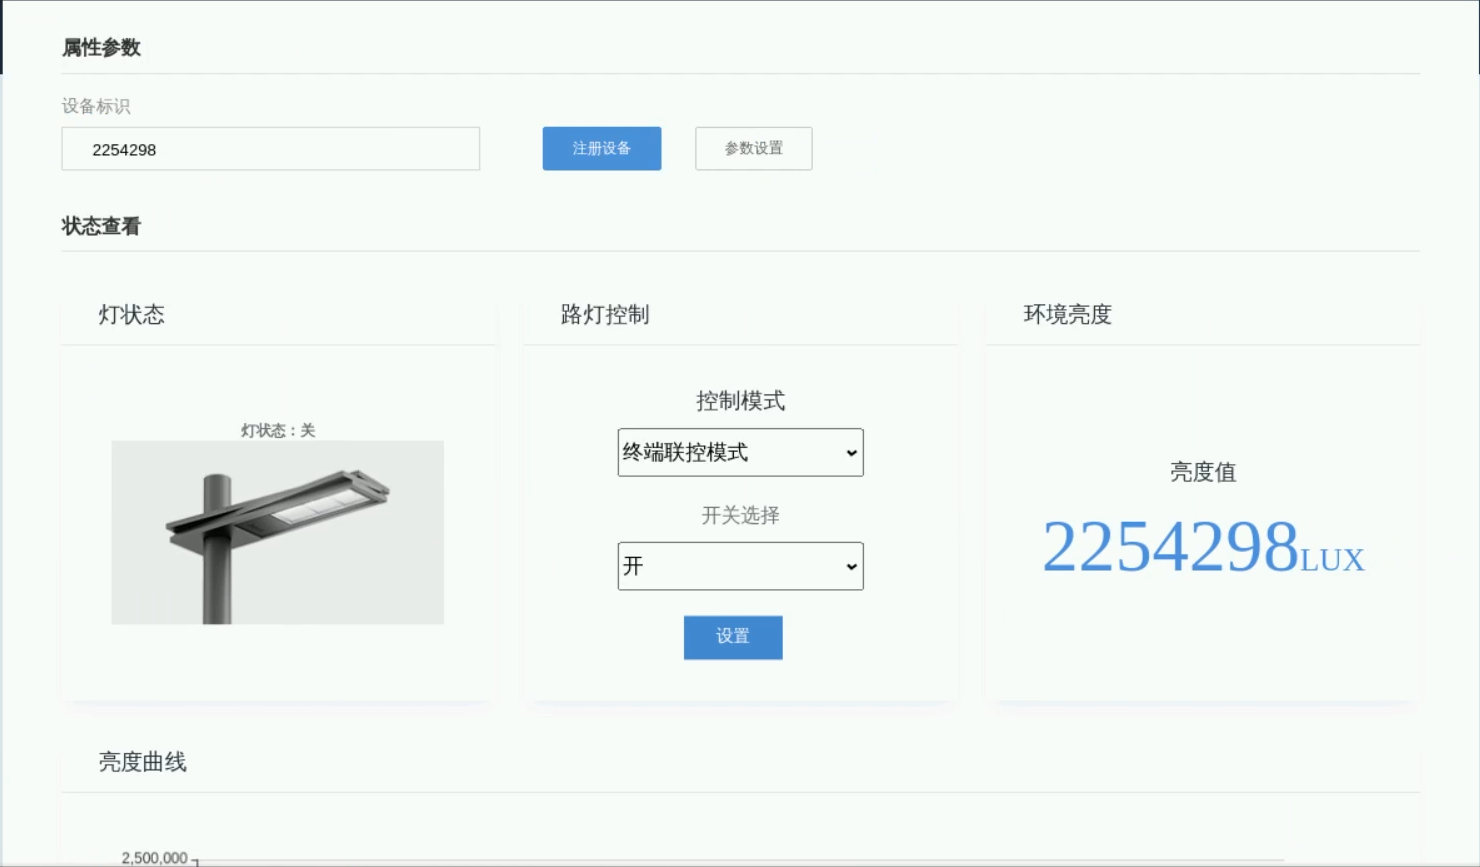
\includegraphics[width=\textwidth]{figures/序列 01.00_19_46_52.Still014.png}
\caption{在模拟器中上报设备属性后智慧路灯应用页面}\label{在模拟器中上报设备属性后智慧路灯应用页面}
\end{figure}

\begin{figure}[!htbp]
\centering
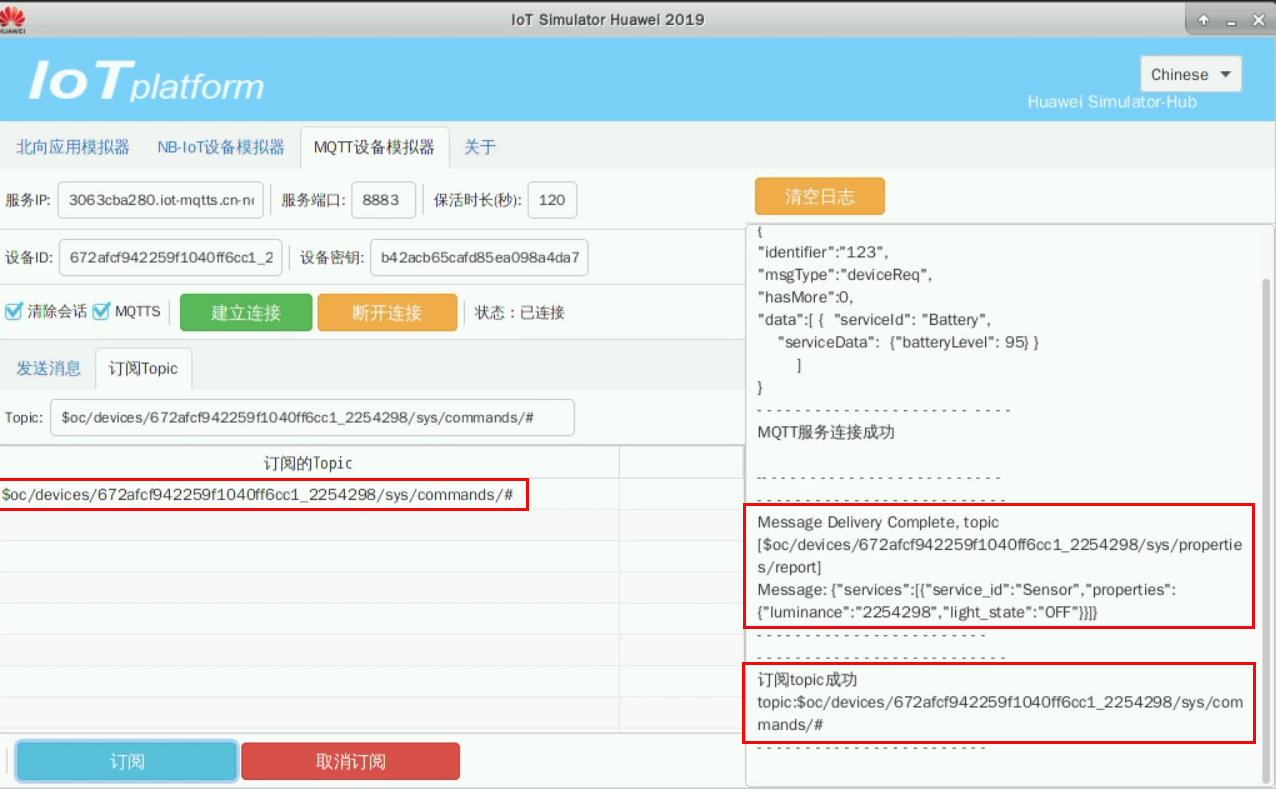
\includegraphics[width=\textwidth]{figures/序列 01.00_20_37_51.Still015.png}
\caption{成功订阅推送方案}\label{成功订阅推送方案}
\end{figure}

\begin{figure}[!htbp]
\centering
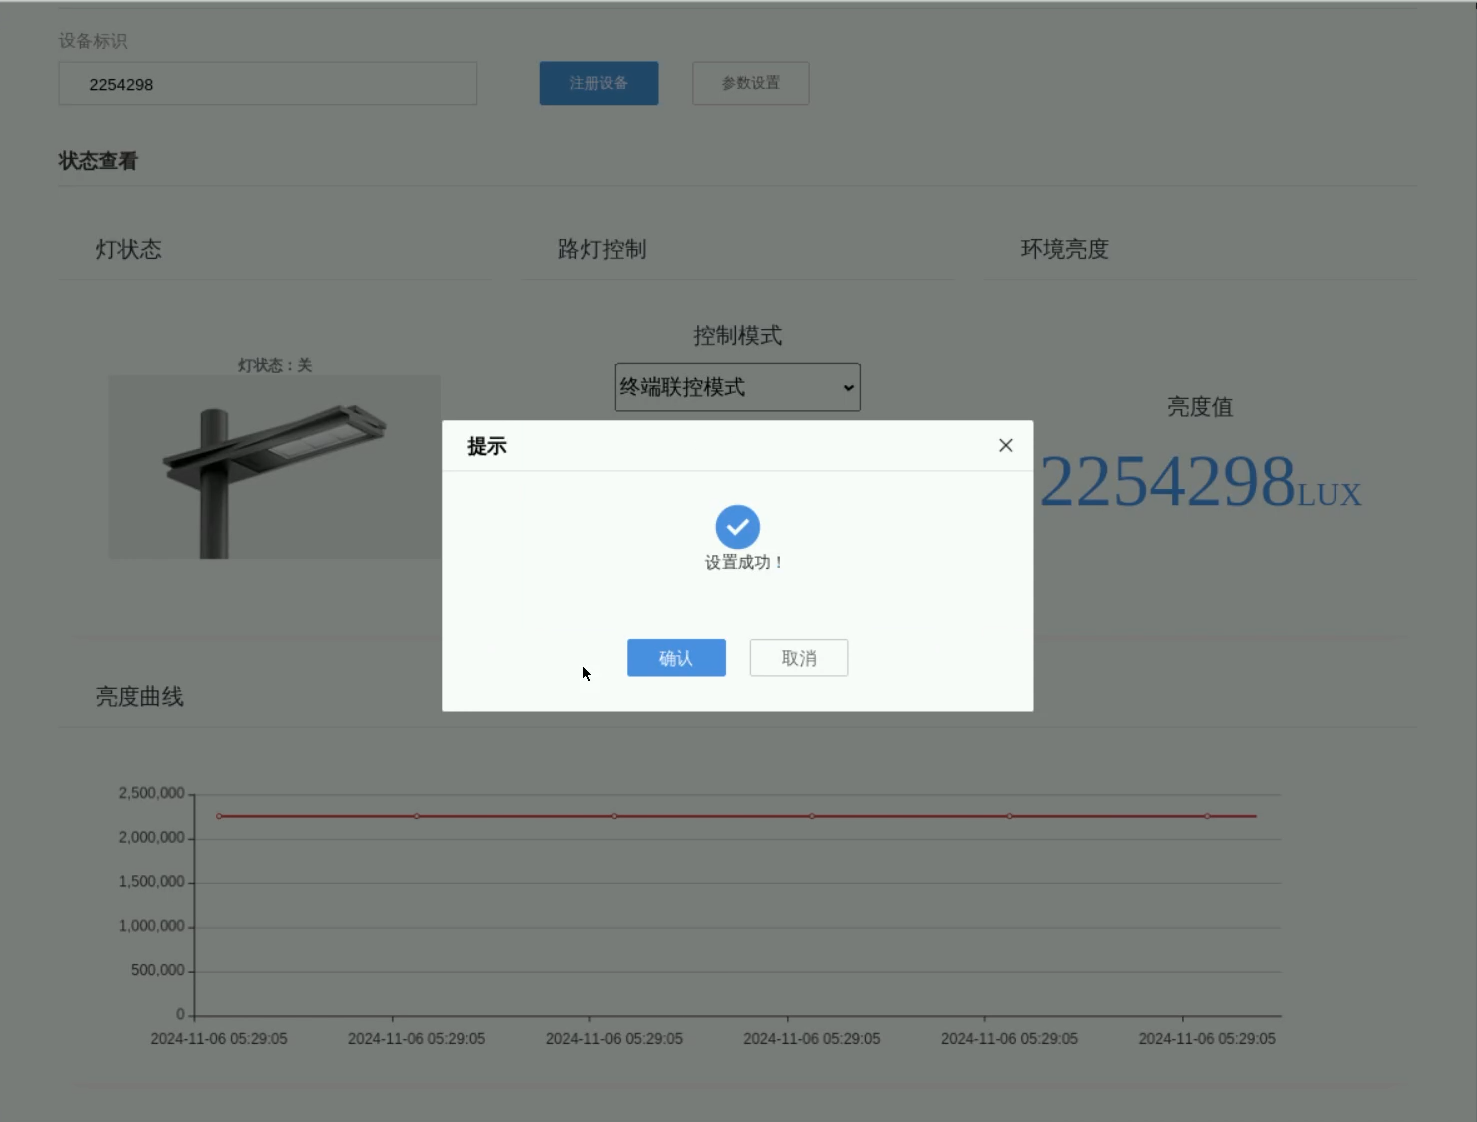
\includegraphics[width=\textwidth]{figures/序列 01.00_21_29_56.Still016.png}
\caption{在智慧路灯应用界面中开启终端联控模式}\label{在智慧路灯应用界面中开启终端联控模式}
\end{figure}

\begin{figure}[!htbp]
\centering
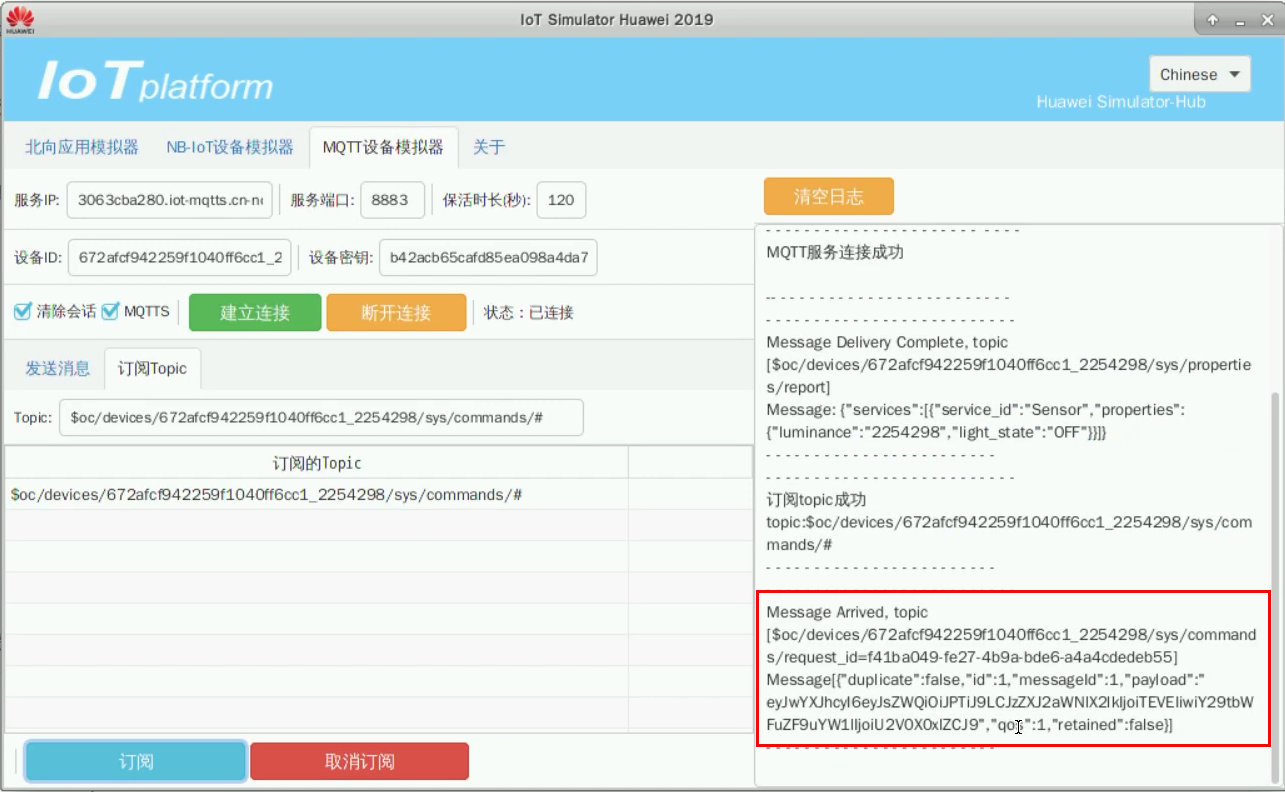
\includegraphics[width=\textwidth]{figures/序列 01.00_21_51_48.Still017.png}
\caption{模拟器中打印日志}\label{模拟器中打印日志}
\end{figure}

\begin{figure}[!htbp]
\centering
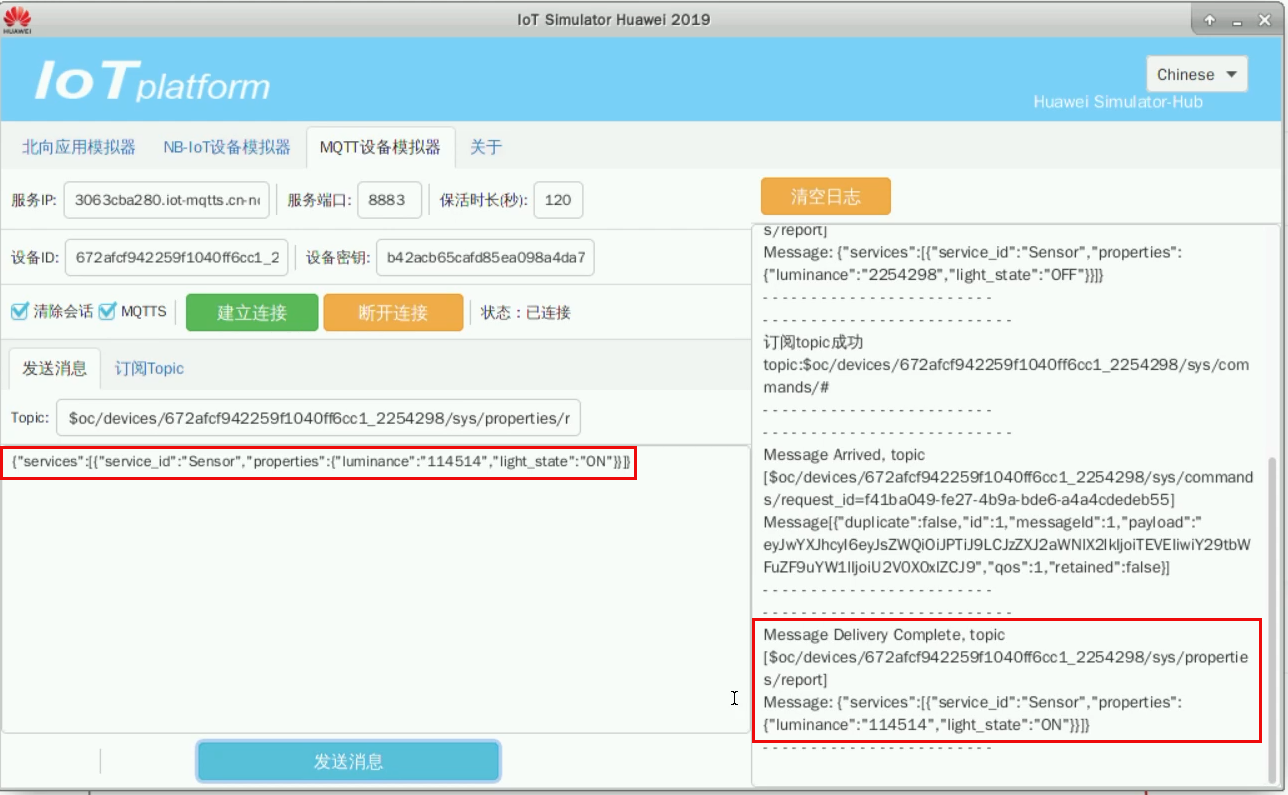
\includegraphics[width=\textwidth]{figures/序列 01.00_23_37_48.Still018.png}
\caption{模拟器中上报设备属性}\label{模拟器中上报设备属性}
\end{figure}

\begin{figure}[!htbp]
\centering
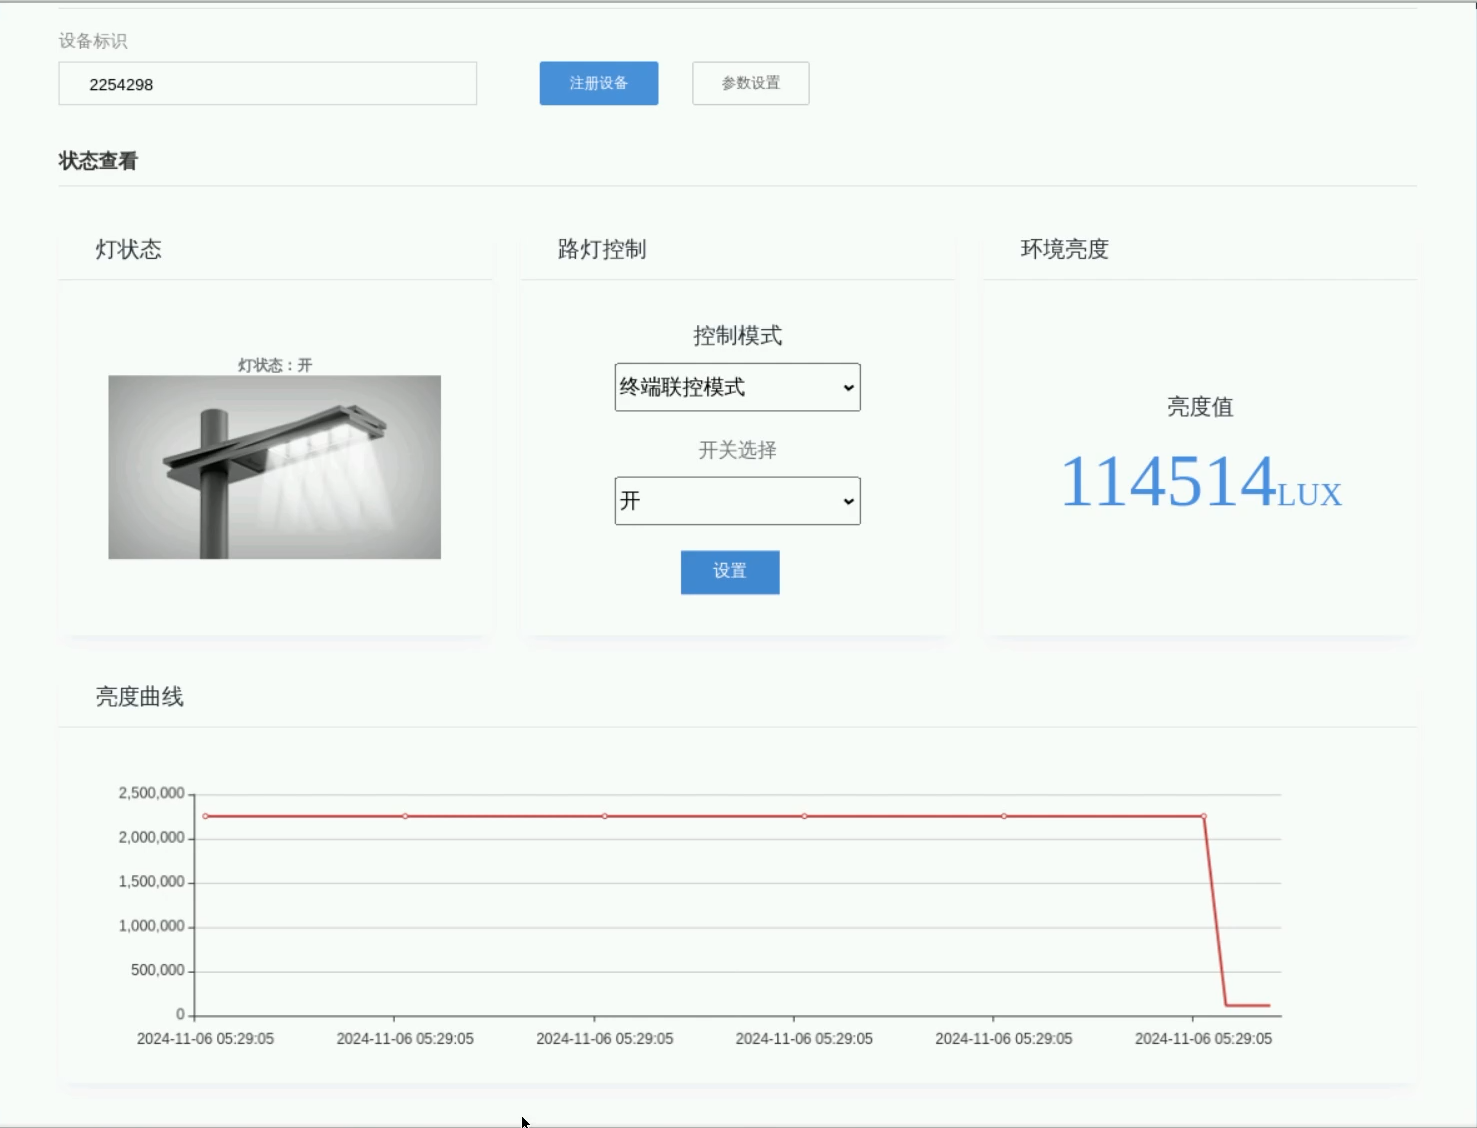
\includegraphics[width=\textwidth]{figures/序列 01.00_23_49_54.Still019.png}
\caption{智慧路灯应用界面中的灯状态与亮度值产生相应变化}\label{智慧路灯应用界面中的灯状态与亮度值产生相应变化}
\end{figure}

\begin{figure}[!htbp]
\centering
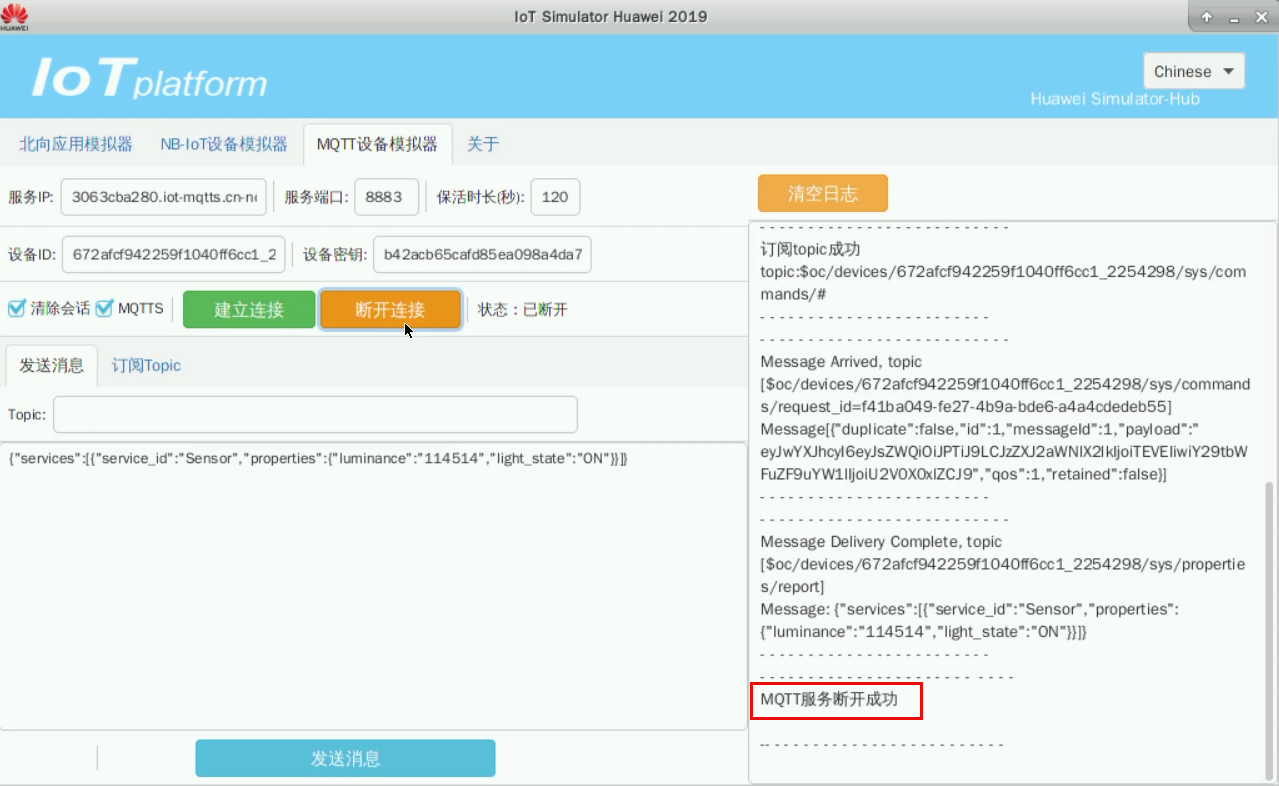
\includegraphics[width=\textwidth]{figures/序列 01.00_23_56_44.Still020.png}
\caption{在模拟器中点击断开连接}\label{在模拟器中点击断开连接}
\end{figure}

\begin{figure}[!htbp]
\centering
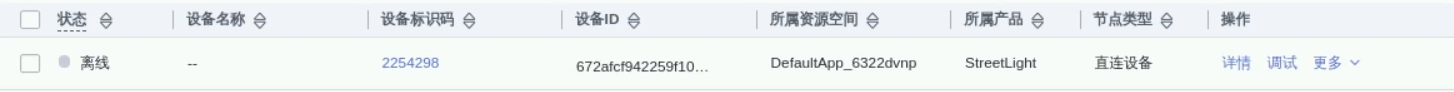
\includegraphics[width=\textwidth]{figures/序列 01.00_24_23_14.Still022.png}
\caption{设备状态改变为离线}\label{设备状态改变为离线}
\end{figure}


\begin{figure}[!htbp]
\centering
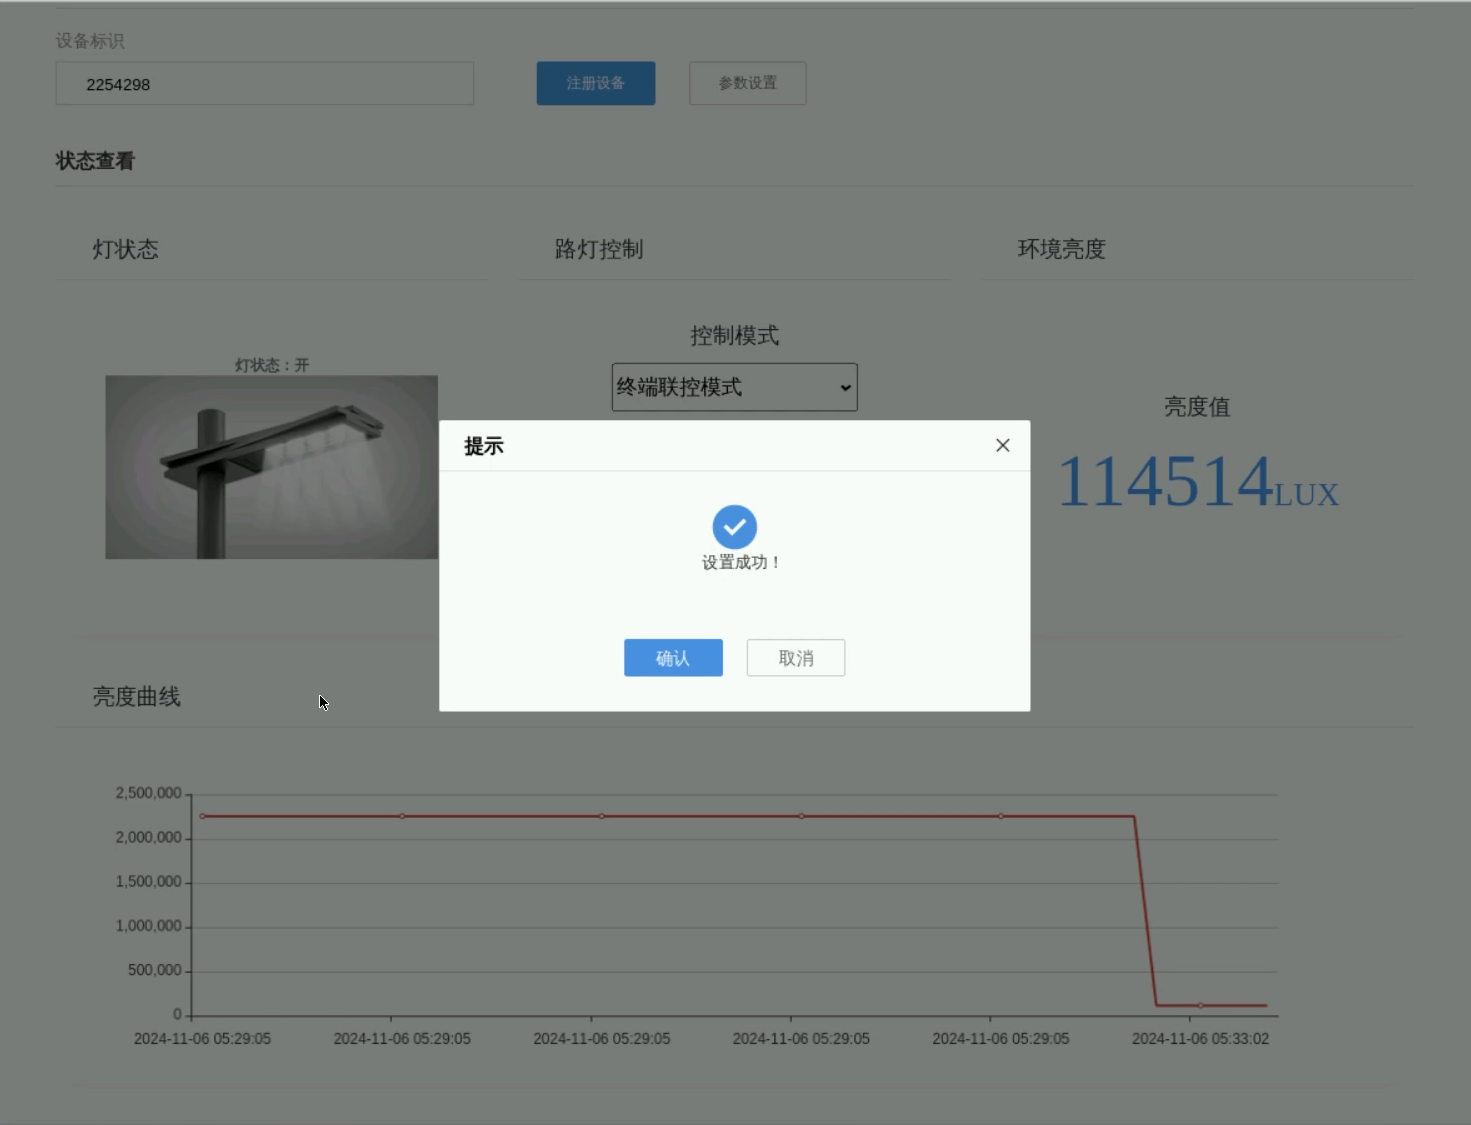
\includegraphics[width=\textwidth]{figures/序列 01.00_24_06_03.Still021.png}
\caption{再次在智慧路灯应用界面中设置终端联控模式}\label{再次在智慧路灯应用界面中设置终端联控模式}
\end{figure}


\begin{figure}[!htbp]
\centering
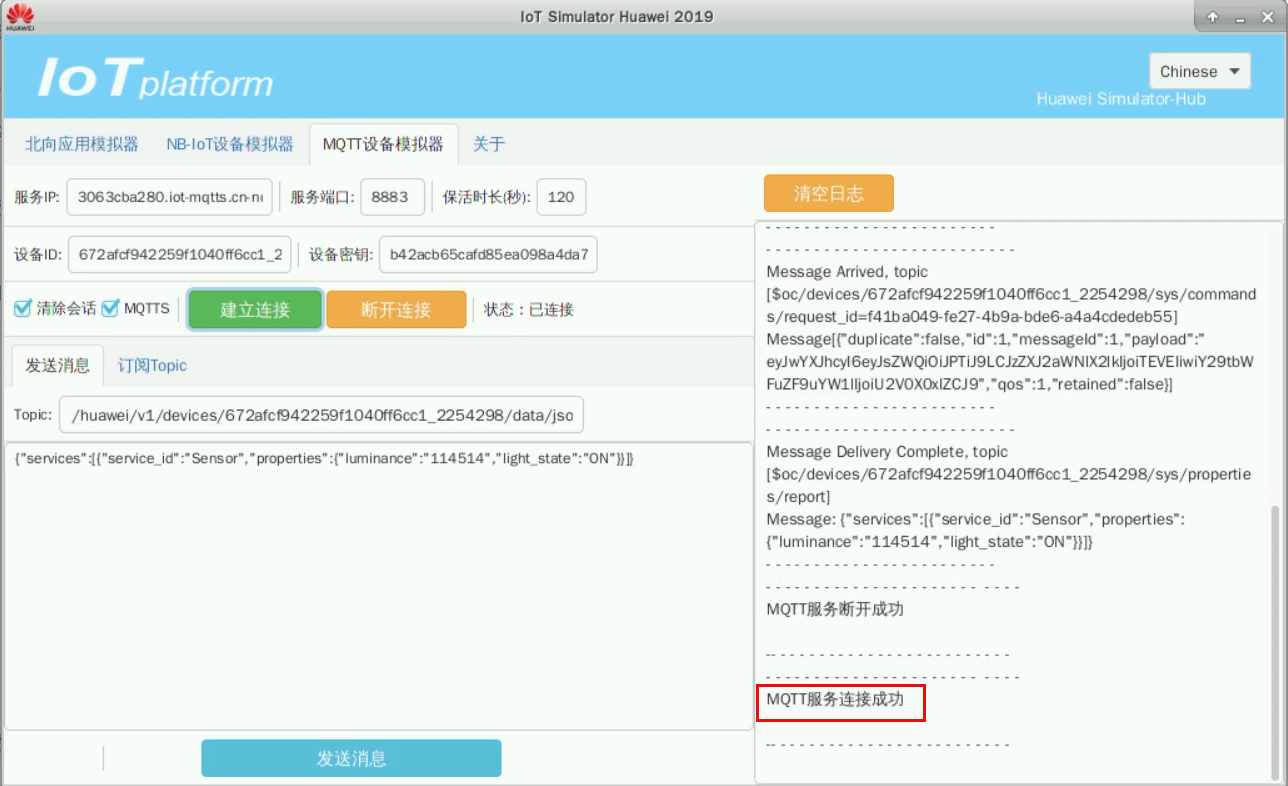
\includegraphics[width=\textwidth]{figures/序列 01.00_24_40_49.Still023.png}
\caption{在模拟器中重新建立连接}\label{在模拟器中重新建立连接}
\end{figure}

\begin{figure}[!htbp]
\centering
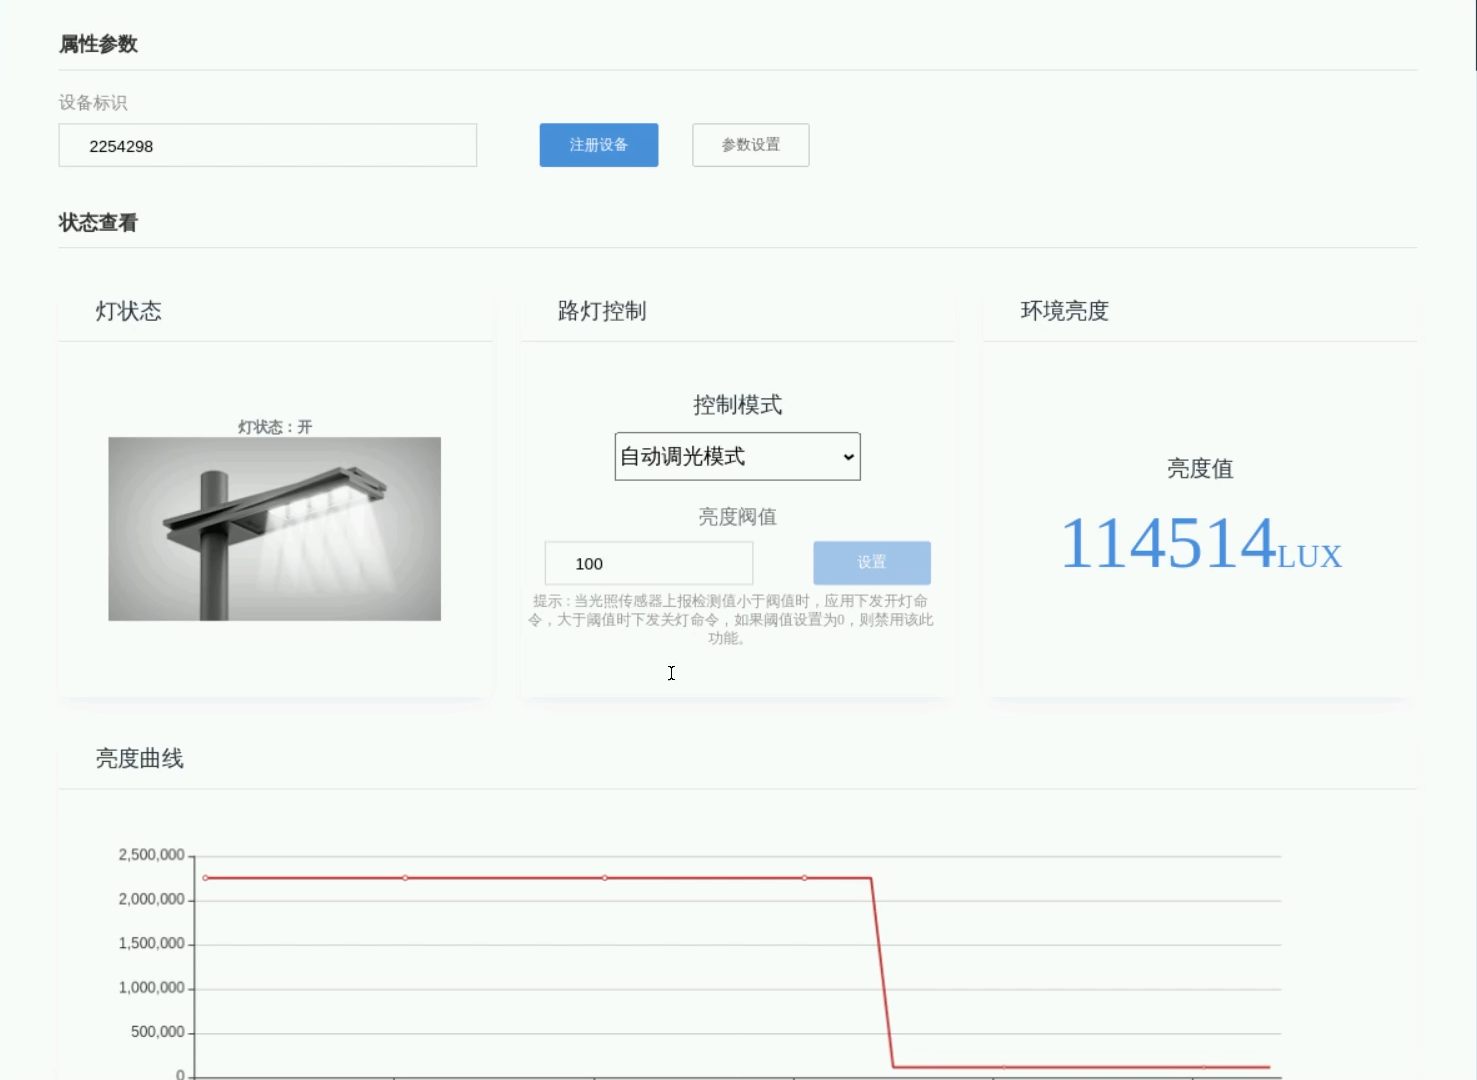
\includegraphics[width=\textwidth]{figures/序列 01.00_25_02_59.Still024.png}
\caption{在智慧路灯应用界面中设置自动调光模式}\label{在智慧路灯应用界面中设置自动调光模式}
\end{figure}

\begin{figure}[!htbp]
\centering
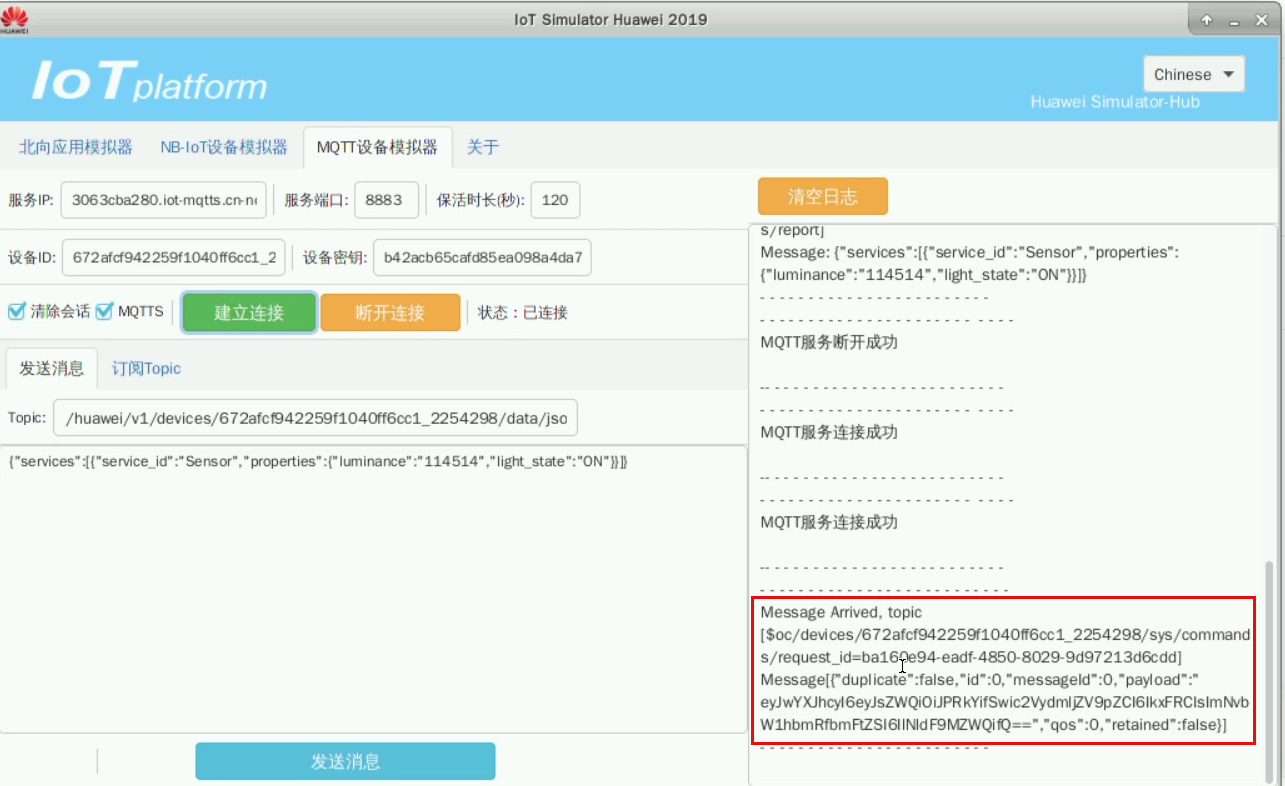
\includegraphics[width=\textwidth]{figures/序列 01.00_25_35_10.Still025.png}
\caption{模拟器中打印相关日志}\label{模拟器中打印相关日志1}
\end{figure}

\begin{figure}[!htbp]
\centering
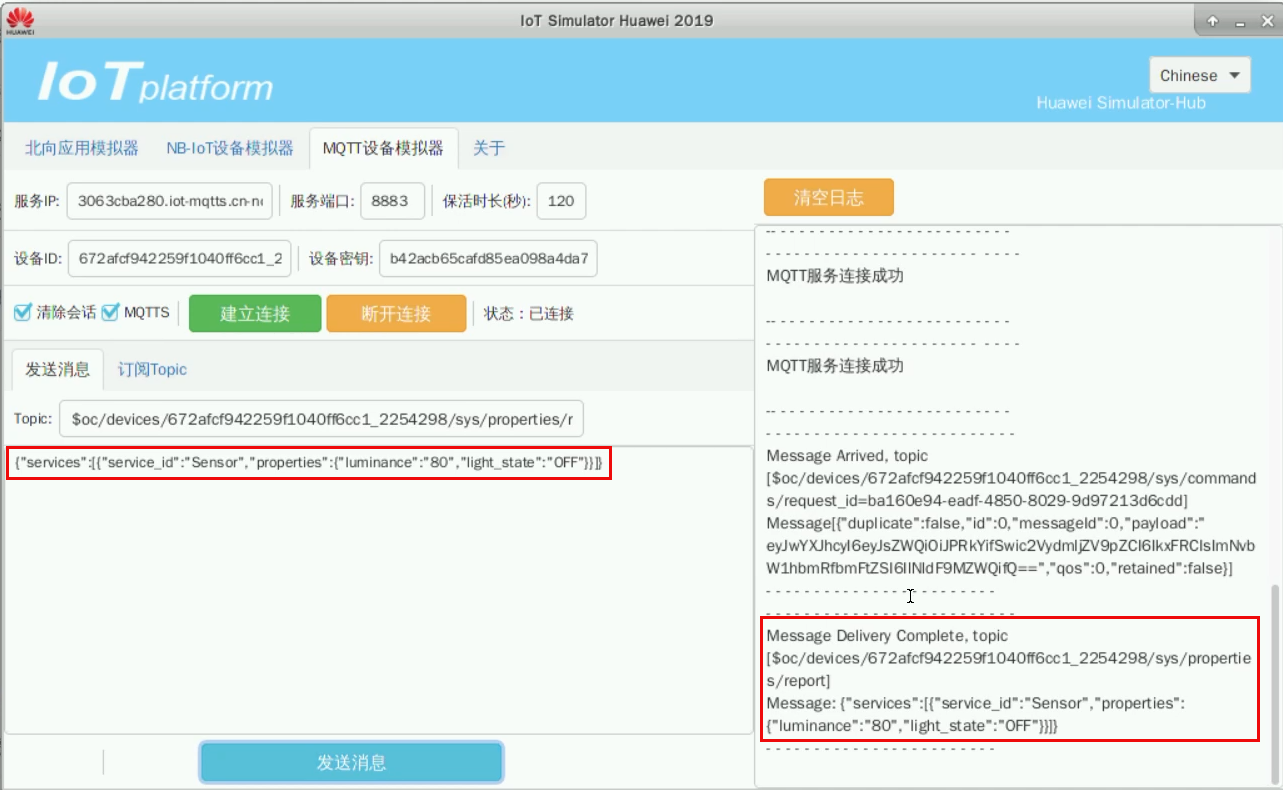
\includegraphics[width=\textwidth]{figures/序列 01.00_26_45_12.Still026.png}
\caption{在模拟器中上报设备属性}\label{在模拟器中上报设备属性}
\end{figure}

\begin{figure}[!htbp]
\centering
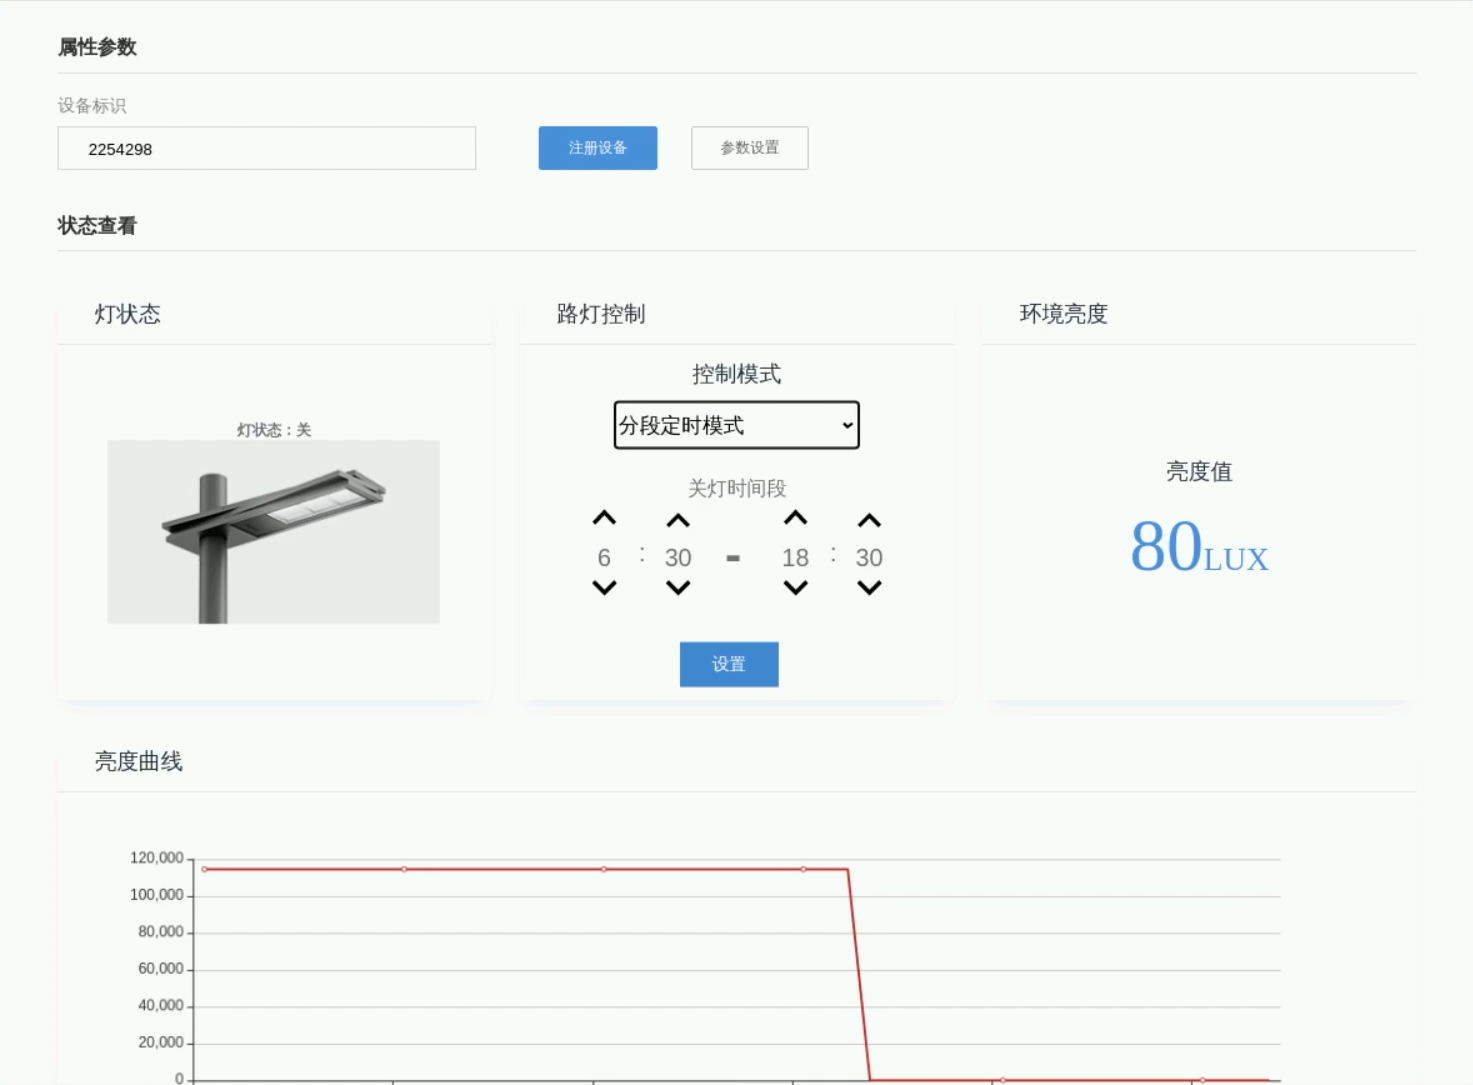
\includegraphics[width=\textwidth]{figures/序列 01.00_28_20_37.Still027.png}
\caption{在智慧路灯应用界面中设置分段定时模式}\label{在智慧路灯应用界面中设置分段定时模式}
\end{figure}

\begin{figure}[!htbp]
\centering
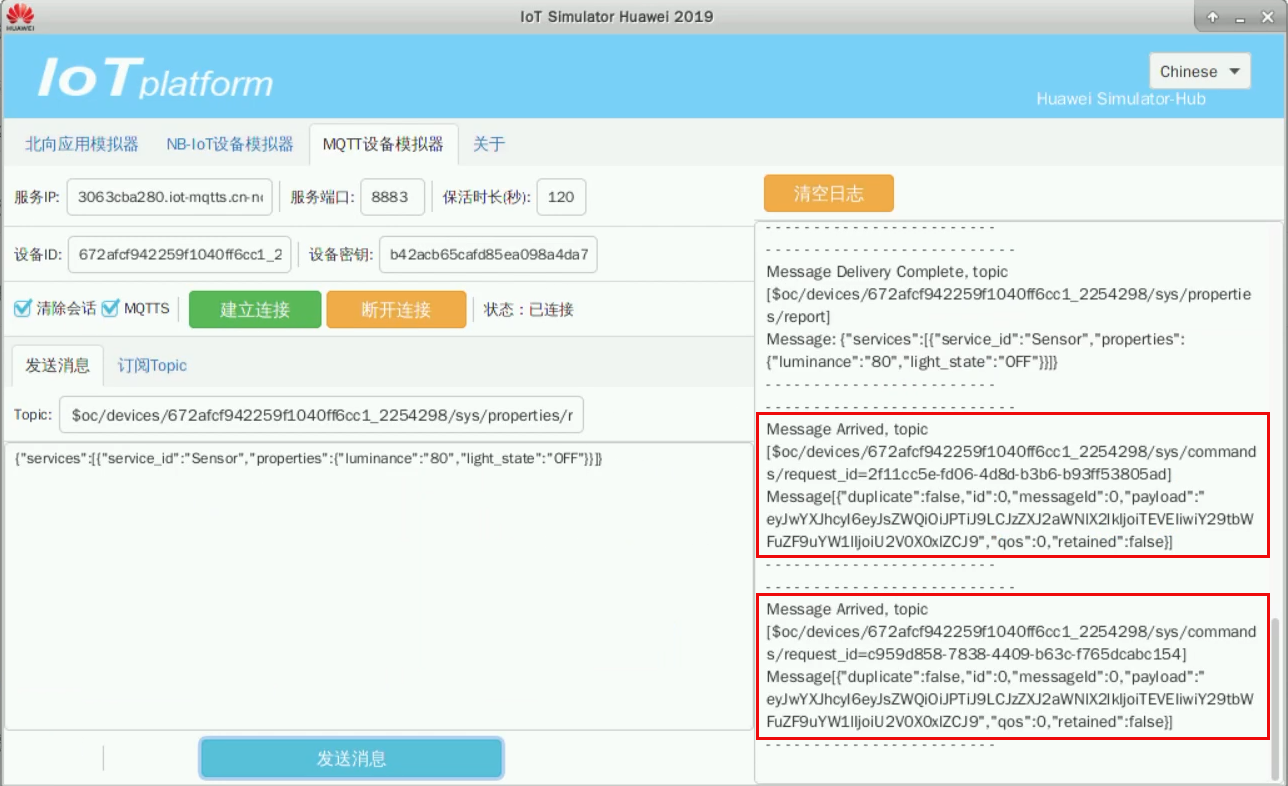
\includegraphics[width=\textwidth]{figures/序列 01.00_28_52_01.Still028.png}
\caption{模拟器中打印相关日志}\label{模拟器中打印相关日志2}
\end{figure}
